\documentclass[12pt,a4paper]{article}
\usepackage[top=2.5cm,bottom=2.5cm,left=3cm,right=2.5cm,headheight=44pt,headsep=12pt,footskip=30pt]{geometry}
\usepackage{fontspec}
\setmainfont{Times New Roman}
\usepackage{amsmath,amssymb}
\usepackage{graphicx}
\usepackage{float}
\usepackage{booktabs}
\usepackage{array}
\usepackage{tabularx}
\usepackage[table]{xcolor}
\usepackage{enumitem}
\usepackage{fancyhdr}
\usepackage{lastpage}
\usepackage{caption}
\usepackage{listings}
\usepackage[most]{tcolorbox}
\usepackage{tikz}
\usetikzlibrary{positioning,arrows.meta,shapes.geometric,calc}
\usepackage{microtype}
\usepackage{needspace}
\usepackage[hidelinks]{hyperref}
\usepackage{setspace}
\setstretch{1.15}

\newcommand{\namakelompok}{Profil2Spartans}
\newcommand{\nomorkelompok}{15}
\newcommand{\semester}{Semester I Tahun 2026/2027}
\newcommand{\repourl}{https://github.com/longlivephos/algeo26-tb1-profil2spartans}
\newcommand{\isi}[1]{\textcolor{red}{[#1]}}
\renewcommand{\contentsname}{Daftar Isi}
\renewcommand{\listfigurename}{Daftar Gambar}
\renewcommand{\listtablename}{Daftar Tabel}
\renewcommand{\figurename}{Gambar}
\renewcommand{\tablename}{Tabel}
\renewcommand{\refname}{Daftar Pustaka}

\newlength{\tinggilogo}\setlength{\tinggilogo}{1.1cm}
\newlength{\jaraklogo}\setlength{\jaraklogo}{9pt}
\newcommand{\logoheader}{%
  
\includegraphics[height=\tinggilogo]{gambar/logo-itb.png}\hspace{\jaraklogo}%
  
\includegraphics[height=\tinggilogo]{gambar/logo-stei.png}\hspace{\jaraklogo}%
  
\includegraphics[height=\tinggilogo,width=1.9cm,keepaspectratio]{gambar/sampul-kelompok.png}}
\newcommand{\teksheader}{%
  \footnotesize\setstretch{1.0}%
  IF2123 Aljabar Linier dan Geometri\\
  Laporan Tugas Besar 1\\
  \semester}
\pagestyle{fancy}
\fancyhf{}
\fancyhead[C]{\parbox[b]{\headwidth}{%
  \begin{minipage}[c]{0.55\headwidth}\raggedright\logoheader\end{minipage}%
  \begin{minipage}[c]{0.45\headwidth}\raggedleft\teksheader\end{minipage}%
  \par\vspace{-3pt}\mbox{}}}
\fancyfoot[L]{\small Kelompok \namakelompok}
\fancyfoot[R]{\small Halaman \thepage{} dari \pageref*{LastPage}}
\renewcommand{\headrulewidth}{0.5pt}
\renewcommand{\footrulewidth}{0.5pt}

\definecolor{abuhead}{gray}{0.93}
\definecolor{komentar}{RGB}{34,120,60}
\definecolor{hijaubox}{RGB}{42,140,90}

\newtcolorbox{kelas}[1]{breakable, enhanced, sharp corners,
  before={\par\vspace{6pt}\needspace{8\baselineskip}\noindent}, after={\par\vspace{6pt}},
  colback=white, colframe=black!75, boxrule=0.5pt,
  left=6pt, right=6pt, top=0pt, bottom=6pt,
  before upper={\setlength{\parskip}{2pt}\small},
  title={\normalsize\bfseries #1}, fonttitle=\bfseries,
  colbacktitle=abuhead, coltitle=black, titlerule=0.5pt}
\newcommand{\kbag}[1]{\par\vspace{5pt}\noindent
  \colorbox{abuhead}{\parbox{\dimexpr\linewidth-2\fboxsep}{\bfseries #1}}\par\vspace{2pt}}
\newcommand{\sig}[1]{\par\noindent\texttt{#1}}
\newcommand{\kom}[1]{\par\noindent\hspace*{1em}{\color{komentar}// #1}}

\newtcolorbox{kasus}{breakable, enhanced, sharp corners,
  before={\par\vspace{6pt}\noindent}, after={\par\vspace{6pt}},
  colback=white, colframe=black!75, boxrule=0.5pt,
  left=6pt, right=6pt, top=0pt, bottom=6pt,
  before upper={\setlength{\parskip}{4pt}}}
  
\newcommand{\ubag}[1]{\par\vspace{4pt}\noindent
  \colorbox{abuhead}{\parbox{\dimexpr\linewidth-2\fboxsep}{\centering\bfseries #1}}\par\vspace{2pt}}

\newtcolorbox{komentar}[1]{enhanced, arc=4pt, boxrule=0.6pt,
  colback=hijaubox!8, colframe=hijaubox!70!black,
  attach boxed title to top left={xshift=6pt, yshift=-3mm},
  boxed title style={sharp corners, colback=hijaubox, boxrule=0pt},
  fonttitle=\bfseries\small\color{white}, title={#1}, top=5mm}

\lstset{basicstyle=\ttfamily\footnotesize, columns=fullflexible,
  breaklines=true, frame=single, framerule=0.3pt,
  backgroundcolor=\color{black!3}, showstringspaces=false}

\newcommand{\tangkapan}[1]{%
  \begin{center}
    \includegraphics[width=0.9\linewidth,height=0.85\textheight,keepaspectratio]{gambar/#1}   \end{center} }

\setlength{\parindent}{0pt}
\setlength{\parskip}{6pt}
\setlength{\emergencystretch}{3em}

\begin{document}

\begin{titlepage}
\centering
\vspace*{0.5cm}
{\LARGE\bfseries Laporan Tugas Besar 1\par}
\vspace{8pt}
{\large IF2123 ALJABAR LINIER DAN GEOMETRI\par}
\vspace{2pt}
{\normalsize SISTEM PERSAMAAN LINIER, DETERMINAN, DAN PENERAPANNYA\par}
\vspace{2pt}
{\normalsize \MakeUppercase{\semester}\par}

\vspace{1.2cm}

\includegraphics[width=0.78\textwidth,height=8.5cm,keepaspectratio]{gambar/sampul-kelompok.png}
\vspace{1.0cm}

{\normalsize Disusun oleh Kelompok \nomorkelompok{} \textbf{\namakelompok}:\par}
\vspace{6pt}
\begin{tabular}{l@{\hspace{2cm}}l}
 Neysa Alya Mukhbita & 13525080 \\
 Jonathan Lewie & 13525136 \\
 Cathrine Angel Siburian & 13525138 \\
\end{tabular}

\vfill
{\normalsize LABORATORIUM ILMU DAN REKAYASA KOMPUTASI\\[2pt]
PROGRAM STUDI TEKNIK INFORMATIKA\\[2pt]
SEKOLAH TEKNIK ELEKTRO DAN INFORMATIKA\\[2pt]
INSTITUT TEKNOLOGI BANDUNG\par}
\end{titlepage}

\setcounter{page}{1}
\tableofcontents
\clearpage
\listoftables
\listoffigures
\clearpage


\section{Pendahuluan}

\subsection{Deskripsi Masalah}

Mitya, peneliti muda di Snezhnaya, sedang menjalankan Proyek Stuzha untuk mengendalikan fluktuasi energi ekstrem di Teyvat. Masalahnya sederhana tapi menghambat: ia masih memakai kalkulator saku tua yang sering error begitu diberi perhitungan berdimensi tinggi. Lewat Adventurers' Guild, Mitya meminta dibuatkan alat hitung otomatis yang sanggup menyelesaikan sistem matriks dan persamaan linier.

Alat tersebut harus bisa menyelesaikan sistem persamaan linier (SPL), menghitung determinan, dan mencari matriks balikan. Alat yang sama juga dipakai untuk memetakan data eksperimen, sehingga perlu fitur interpolasi polinomial, interpolasi \textit{natural cubic spline}, dan regresi spline kubik.
\subsection{Latar Belakang}

Sebagian besar permasalahan yang dibahas pada tugas ini pada akhirnya berkaitan dengan persoalan penyelesaian SPL. Pada interpolasi polinomial, SPL diperoleh melalui pembentukan matriks Vandermonde. Sementara itu, interpolasi \textit{natural cubic spline} menghasilkan SPL berbentuk tridiagonal, sedangkan regresi spline menggunakan persamaan normal $(X^TX)\beta = X^Ty$. Oleh karena itu, \textit{library} yang dikembangkan disusun secara bertahap, dimulai dari operasi dasar pada matriks melalui kelas \texttt{Matrix}, kemudian dilanjutkan dengan implementasi metode eliminasi, determinan, dan matriks balikan. Metode-metode tersebut selanjutnya menjadi dasar untuk mengembangkan fitur interpolasi dan regresi.

\subsection{Tujuan}

Tugas besar ini memiliki beberapa tujuan sebagai berikut:
\begin{enumerate}[nosep]
\item mengimplementasikan secara mandiri dalam Java berbagai metode penyelesaian SPL, yaitu eliminasi Gauss, Gauss-Jordan, matriks balikan, dan kaidah Cramer, serta metode perhitungan determinan, matriks balikan, interpolasi polinomial, \textit{natural cubic spline}, dan regresi spline kubik;
\item membangun metode-metode tersebut menjadi sebuah \textit{library} yang modular, terdokumentasi, dan dapat digunakan kembali melalui program berbasis CLI maupun GUI;
\item melakukan pengujian terhadap \textit{library} menggunakan kasus-kasus uji yang ditentukan dalam Bab 5 dokumen spesifikasi serta menganalisis hasil yang diperoleh, termasuk mengamati perbedaan hasil antar-metode yang dapat muncul.
\end{enumerate}

\clearpage
\section{Dasar Teori}

\subsection{Sistem Persamaan Linier}

SPL dengan $m$ persamaan dan $n$ variabel dapat ditulis sebagai $Ax = b$, dengan $A$ merupakan matriks koefisien berukuran $m \times n$, $x$ vektor variabel, dan $b$ vektor konstanta. Dalam program, SPL disimpan sebagai matriks \textit{augmented} $[A\,|\,b]$ berukuran $m \times (n+1)$. Sebuah SPL bisa memiliki solusi tunggal, tak hingga banyak solusi, atau tidak memiliki solusi sama sekali.

Ketiga kemungkinan solusi tersebut dapat diketahui melalui rank \cite{anton}. Jika $\operatorname{rank}(A) < \operatorname{rank}([A\,|\,b])$ terdapat baris berbentuk $0 = c$ dengan $c \neq 0$ yang membuat SPL tidak konsisten. Jika kedua rank sama dan bernilai $n$ maka  solusinya tunggal. Jika kedua rank sama tetapi kurang dari $n$ maka terdapat $n - \operatorname{rank}(A)$ variabel bebas dan solusinya ditulis dalam bentuk parametrik.

\subsubsection{Operasi Baris Elementer}

Ketiga operasi baris elementer (OBE) adalawh sebagai berikut tanpa mengubah himpunan solusi SPL:
\begin{enumerate}[nosep]
  \item menukar dua baris;
  \item mengalikan sebuah baris dengan konstanta tidak nol;
  \item menambahkan kelipatan sebuah baris ke baris lain.
\end{enumerate}

\subsubsection{Eliminasi Gauss}

Eliminasi Gauss memakai OBE untuk mengubah $[A\,|\,b]$ menjadi matriks eselon baris. Setiap baris tidak nol diawali angka 1 (satu utama) dan satu utama pada baris di bawahnya selalu terletak lebih ke kanan. Setelah bentuk eselon tercapai, selanjutnya nilai variabel dicari dari baris paling bawah ke atas dengan substitusi mundur:
\[
x_i = b'_i - \sum_{j=i+1}^{n} a'_{ij}\, x_j .
\]

\subsubsection{Eliminasi Gauss-Jordan}

Gauss-Jordan melanjutkan eliminasi Gauss sampai matriks berbentuk eselon baris tereduksi dimana setiap kolom yang memuat satu utama bernilai nol di semua baris lain. Pada bentuk ini solusi dapat langsung dibaca dari kolom terakhir tanpa substitusi mundur.

\subsubsection{\textit{Partial Pivoting}}

Komputer menyimpan bilangan real sebagai \textit{floating point} dengan presisi terbatas (sekitar 16 digit desimal untuk tipe data \texttt{double}). Jika elemen pivot sangat kecil, faktor pengali $a_{ik}/a_{kk}$ menjadi sangat besar dan galat pembulatan ikut membesar. \textit{Partial pivoting} mencegah hal ini dengan memilih baris yang memiliki nilai mutlak terbesar pada kolom yang sedang diproses lalu menukarnya ke posisi pivot.

\subsubsection{Metode Matriks Balikan}

Jika $A$ merupakan matriks berukuran $m$ $x$ $m$ persegi dan memiliki balikan, kedua ruas $Ax = b$ dapat dikalikan dari kiri dengan $A^{-1}$ sehingga
\[
x = A^{-1} b .
\]
Metode ini hanya berlaku untuk SPL dengan jumlah persamaan ($baris$) sama dengan jumlah variabel($kolom$) dan $\det(A) \neq 0$.

\subsubsection{Kaidah Cramer}

Untuk $A$ berukuran $n \times n$ dengan $\det(A) \neq 0$, solusi tunggal SPL adalah
\[
x_k = \frac{\det(A_k)}{\det(A)}, \qquad k = 1, 2, \dots, n,
\]
dengan $A_k$ adalah matriks $A$ yang kolom ke-$k$-nya diganti vektor $b$. Kaidah ini membutuhkan $n+1$ perhitungan determinan, sehingga jauh lebih lambat daripada eliminasi untuk $n$ besar.

\subsection{Determinan Matriks}

Determinan adalah skalar yang dihitung dari matriks persegi $A$ dan ditulis $\det(A)$ atau $|A|$. Matriks persegi memiliki balikan jika dan hanya jika $\det(A) \neq 0$. Matriks yang tidak persegi tidak memiliki determinan. Untuk memperoleh determinan sebuah matriks dapat dilakukan dengan metode berikut ini.

\subsubsection{Metode Reduksi Baris}

Metode ini mengubah $A$ menjadi matriks segitiga atas $U$ dengan OBE, lalu memakai sifat bahwa determinan matriks segitiga sama dengan hasil kali elemen diagonalnya. Pengaruh tiap OBE terhadap determinan harus dicatat, yaitu:
\begin{itemize}[nosep]
  \item menukar dua baris membalik tanda determinan;
  \item mengalikan baris dengan $k$ mengalikan determinan dengan $k$;
  \item menambahkan kelipatan baris ke baris lain tidak mengubah determinan.
\end{itemize}
Jika hanya operasi tukar baris dan penambahan kelipatan yang dipakai, dengan $s$ kali pertukaran baris, maka berlaku :
\[
\det(A) = (-1)^{s} \prod_{i=1}^{n} u_{ii} .
\]

\subsubsection{Metode Ekspansi Kofaktor}

Minor $M_{ij}$ adalah determinan submatriks yang tersisa setelah baris ke-$i$ dan kolom ke-$j$ dihapus. Kofaktornya adalah $C_{ij} = (-1)^{i+j} M_{ij}$. Determinan dapat dihitung dengan ekspansi sepanjang baris ke-$i$ mana pun,
\[
\det(A) = \sum_{j=1}^{n} a_{ij}\, C_{ij},
\]
atau sepanjang kolom mana pun karena $\det(A) = \det(A^T)$. Memilih baris atau kolom dengan elemen nol terbanyak perlu diperhatikan untukmengurangi jumlah minor yang perlu dihitung. Meskipun demikian, kompleksitasnya tetap $O(n!)$ sehingga metode ini hanya praktis untuk matriks kecil.

\subsection{Matriks Balikan}

Balikan dari matriks persegi $A$ adalah matriks $A^{-1}$ yang memenuhi $AA^{-1} = A^{-1}A = I$.

\subsubsection{Metode Augmentasi}

Matriks $A$ digabung dengan matriks identitas menjadi $[A\,|\,I]$, lalu direduksi dengan Gauss-Jordan. Jika bagian kiri berhasil menjadi $I$ maka bagian kanan adalah $A^{-1}$:
\[
[A\,|\,I] \xrightarrow{\text{OBE}} [I\,|\,A^{-1}] .
\]
Jika selama proses muncul kolom tanpa pivot tak nol, dapat diketahui bahwa $A$ adalah matriks singular dan tidak memiliki balikan.

\subsubsection{Metode Adjoin}

Matriks kofaktor $C$ berisi seluruh kofaktor $C_{ij}$. Adjoin dari $A$ adalah transpose matriks kofaktor, $\operatorname{adj}(A) = C^T$. Balikan dihitung dengan
\[
A^{-1} = \frac{1}{\det(A)}\, \operatorname{adj}(A), \qquad \det(A) \neq 0 .
\]

\subsection{Interpolasi Polinomial}

Diberikan $n+1$ titik $(x_0, y_0), \dots, (x_n, y_n)$ dengan nilai $x_i$ berbeda, terdapat tepat satu polinomial berderajat paling tinggi $n$,
\[
P_n(x) = a_0 + a_1 x + a_2 x^2 + \dots + a_n x^n ,
\]
yang melalui semua titik tersebut. Substitusi setiap titik menghasilkan SPL $Va = y$ dengan $V$ matriks Vandermonde:
\[
\begin{bmatrix}
1 & x_0 & x_0^2 & \cdots & x_0^n \\
1 & x_1 & x_1^2 & \cdots & x_1^n \\
\vdots & \vdots & \vdots & \ddots & \vdots \\
1 & x_n & x_n^2 & \cdots & x_n^n
\end{bmatrix}
\begin{bmatrix} a_0 \\ a_1 \\ \vdots \\ a_n \end{bmatrix}
=
\begin{bmatrix} y_0 \\ y_1 \\ \vdots \\ y_n \end{bmatrix}.
\]
Matriks Vandermonde memiliki balikan selama semua $x_i$ berbeda. Namun, matriks ini cepat menjadi \textit{ill-conditioned} ketika jumlah titik bertambah atau nilai $x_i$ berdekatan, sehingga koefisien yang dihasilkan rentan terhadap galat pembulatan. Setelah koefisien diperoleh, $P_n(x_t)$ dapat dievaluasi untuk sembarang $x_t$ di dalam domain $[x_0, x_n]$.

\subsection{\textit{Natural Cubic Spline Interpolation}}

Polinomial berderajat tinggi cenderung berosilasi di dekat ujung interval. Spline kubik menghindari batas interval tersebut dengan memakai polinomial kubik terpisah pada setiap subinterval $[x_j, x_{j+1}]$, $j = 0, \dots, n-1$:
\[
S_j(x) = a_j + b_j (x - x_j) + c_j (x - x_j)^2 + d_j (x - x_j)^3 .
\]
Ada $4n$ koefisien yang dicari. Syaratnya, kurva harus melalui semua titik, nilai, turunan pertama, dan turunan kedua kontinu di setiap simpul dalam. Syarat-syarat ini akan menghasilkan $4n - 2$ persamaan. Dua persamaan sisanya berasal dari syarat batas natural, yaitu turunan kedua di kedua ujung bernilai nol:
\[
S''(x_0) = S''(x_n) = 0 .
\]

\subsubsection{Sistem Tridiagonal}

Dengan $h_j = x_{j+1} - x_j$ dan $a_j = y_j$, seluruh syarat di atas dapat direduksi menjadi SPL yang hanya melibatkan $c_0, \dots, c_n$ \cite{burden}:
\[
h_{j-1}\, c_{j-1} + 2(h_{j-1} + h_j)\, c_j + h_j\, c_{j+1}
= \frac{3}{h_j}(a_{j+1} - a_j) - \frac{3}{h_{j-1}}(a_j - a_{j-1}),
\quad j = 1, \dots, n-1,
\]
ditambah $c_0 = 0$ dan $c_n = 0$ dari syarat batas natural. Setiap persamaan hanya melibatkan tiga variabel yang bersebelahan sehingga matriks koefisiennya tridiagonal dan dominan diagonal. Matriks seperti ini selalu memiliki balikan sehingga SPL-nya selalu memiliki solusi tunggal.

Setelah semua $c_j$ diketahui, koefisien lain dihitung dengan
\[
b_j = \frac{a_{j+1} - a_j}{h_j} - \frac{h_j}{3}(2c_j + c_{j+1}), \qquad
d_j = \frac{c_{j+1} - c_j}{3h_j} .
\]
Karena $S_j''(x_j) = 2c_j$, turunan kedua pada knot ke-$j$ adalah $M_j = 2c_j$. Syarat batas natural $M_0 = M_n = 0$ setara dengan $c_0 = c_n = 0$.

\subsection{Regresi Spline Kubik}

Regresi spline tidak mengharuskan kurva melalui setiap titik. Kurva dicari sedemikian rupa sehingga jumlah kuadrat galatnya minimum. Kurva tersusun atas potongan polinomial yang tersambung pada knot $\xi_1 < \xi_2 < \dots < \xi_K$.

\subsubsection{\textit{Truncated Power Basis}}

Spline berderajat $d$ dengan $K$ knot dapat dinyatakan sebagai kombinasi linier dari $M = d + 1 + K$ fungsi basis \cite{hastie}:
\[
f(x) = \sum_{j=0}^{d} \beta_j x^j + \sum_{k=1}^{K} \beta_{d+k}\, (x - \xi_k)_+^{d},
\qquad
(u)_+ = \max(0, u) .
\]
Untuk spline kubik ($d = 3$), basisnya adalah $1, x, x^2, x^3$ ditambah $(x - \xi_k)_+^3$ untuk setiap knot, sehingga $M = 4 + K$. Fungsi $(x - \xi_k)_+^3$ bernilai nol di kiri knot dan turunan pertama serta keduanya kontinu di $\xi_k$ sehingga $f$ otomatis kontinu hingga turunan kedua tanpa persamaan tambahan. Untuk $d = 1$, basis $(x - \xi_k)_+$ menghasilkan garis patah yang tersambung di setiap knot.

\subsubsection{Matriks Desain dan Persamaan Normal}

Untuk $N$ titik data, setiap baris matriks desain $X \in \mathbb{R}^{N \times M}$ berisi nilai semua fungsi basis di $x_i$ dan model ditulis $y = X\beta + \epsilon$. Jika $N > M$, SPL $X\beta = y$ umumnya tidak konsisten. Solusi kuadrat terkecil $\hat\beta$ adalah vektor yang membuat $X\hat\beta$ menjadi proyeksi ortogonal $y$ ke ruang kolom $X$. Syaratnya, vektor sisa tegak lurus terhadap semua kolom $X$:
\[
X^T(y - X\hat\beta) = 0
\quad\Longrightarrow\quad
(X^TX)\hat\beta = X^Ty .
\]
Persamaan terakhir disebut persamaan normal. Jika kolom-kolom $X$ bebas linier, $X^TX$ simetris definit positif dan $\hat\beta$ tunggal. Syarat ini gagal jika jumlah titik kurang dari $M$ atau jika ada selang antar-knot yang tidak berisi cukup titik data tersebut.

Persamaan normal memiliki bilangan kondisi kira-kira kuadrat dari bilangan kondisi $X$. Kolom $x^3$ yang bernilai besar di samping kolom $1$ yang bernilai kecil membuat $X^TX$ mudah menjadi \textit{ill-conditioned}. Salah satu cara umum menanganinya adalah menskalakan $x$ ke rentang $[-1, 1]$ sebelum membentuk $X$.

\clearpage
\section{Implementasi}

Program dikembangkan menggunakan Java 17 dan dibangun dengan Apache Maven. Kode sumber disimpan di folder \texttt{src/main/java/algeo}, sedangkan kode untuk pengujian berada di folder \texttt{test}. Program dibagi menjadi tiga bagian utama, yaitu \textit{library} perhitungan, bagian masukan-keluaran (\texttt{io}), serta antarmuka pengguna berupa CLI dan GUI. \textit{Dependency} antarbagian dibuat satu arah, sehingga CLI dan GUI dapat menggunakan \textit{library} perhitungan, tetapi \textit{library} tidak bergantung pada kode \textit{interface}. CLI dan GUI juga menggunakan implementasi perhitungan yang sama.


\subsection{Struktur Folder dan Arsitektur}

\begin{lstlisting}
src/main/java/algeo/
|-- App.java                  titik masuk program (GUI atau CLI)
|-- core/
|   |-- matrix/               Matrix, MatrixException
|   |-- util/                 Toleransi, NumberFormatter, DecimalParser
|   |-- spl/                  GaussEliminationSolver, GaussJordan,
|   |                         InverseMethod, Cramer, SPLResult, ...
|   |-- interpolasi/          NaturalCubicSpline, InterpolasiResult, ...
|   `-- regression/           SplineRegression, RegressionOutput
|-- determinant/              OBE, Kofaktor
|-- inverse/                  Augmentasi, Adjoin, InverseResult, ...
|-- interpolasipolinomial/    Interpolasi
|-- io/                       MatrixReader, OutputWriter
|-- modules/                  menu dan submenu CLI
`-- gui/                      tampilan Swing
\end{lstlisting}

Gambar~\ref{fig:arsitektur} menunjukkan hubungan antar paket dalam program, dengan panah yang menunjukkan penggunaan antar paket. Kelas \texttt{Matrix} menjadi dasar yang digunakan oleh paket-paket lainnya. Fitur seperti interpolasi dan regresi memanfaatkan solver SPL serta metode matriks balikan yang telah tersedia.

\begin{figure}[H]
\centering
\begin{adjustbox}{max width=\textwidth}
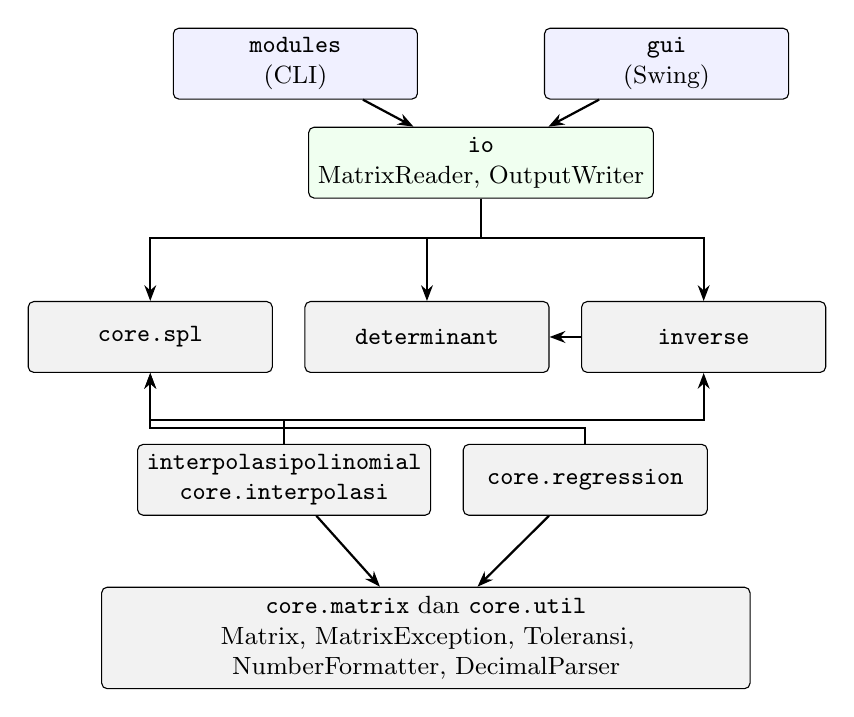
\begin{tikzpicture}[
  kotak/.style={draw, rounded corners=2pt, minimum width=3.1cm, minimum height=0.9cm, align=center, font=\small},
  ui/.style={kotak, fill=blue!6},
  core/.style={kotak, fill=gray!10},
  panah/.style={-{Stealth[length=2mm]}, thick}
]
\node[ui] (cli) {\texttt{modules}\\(CLI)};
\node[ui, right=1.6cm of cli] (gui) {\texttt{gui}\\(Swing)};
\node[kotak, fill=green!6, below=0.8cm of $(cli)!0.5!(gui)$] (io) {\texttt{io}\\MatrixReader, OutputWriter};
\node[core, below=1.3cm of io, xshift=-4.2cm] (spl) {\texttt{core.spl}};
\node[core, right=0.4cm of spl] (det) {\texttt{determinant}};
\node[core, right=0.4cm of det] (inv) {\texttt{inverse}};
\node[core, below=0.9cm of spl, xshift=1.7cm] (itp) {\texttt{interpolasipolinomial}\\\texttt{core.interpolasi}};
\node[core, right=0.4cm of itp] (reg) {\texttt{core.regression}};
\node[core, below=0.9cm of itp, xshift=1.8cm, minimum width=6cm, text width=8cm] (mat) {\texttt{core.matrix} dan \texttt{core.util}\\Matrix, MatrixException, Toleransi,\\NumberFormatter, DecimalParser};
\draw[panah] (cli) -- (io);
\draw[panah] (gui) -- (io);
\draw[panah] (io.south) -- ++(0,-0.5) -| (spl.north);
\draw[panah] (io.south) -- ++(0,-0.5) -| (det.north);
\draw[panah] (io.south) -- ++(0,-0.5) -| (inv.north);
\draw[panah] (inv) -- (det);
\draw[panah] (itp.north) -- ++(0,0.3) -| (inv.south);
\draw[panah] (itp.north) -- ++(0,0.3) -| (spl.south);
\draw[panah] (reg.north) -- ++(0,0.2) -| (spl.south);
\draw[panah] (itp) -- (mat);
\draw[panah] (reg) -- (mat);
\end{tikzpicture}
\end{adjustbox}
\caption{Hubungan antarpaket program}
\label{fig:arsitektur}
\end{figure}

Beberapa ketergantungan antarmetode yang ditunjukkan pada gambar meliputi interpolasi polinomial yang menggunakan \texttt{Augmentasi} untuk memperoleh balikan matriks Vandermonde, serta \textit{natural cubic spline} yang memanfaatkan \texttt{GaussJordan} dalam menyelesaikan SPL tridiagonal. Pada regresi spline, persamaan normal diselesaikan menggunakan \texttt{GaussEliminationSolver}, sementara \texttt{Adjoin} menggunakan \texttt{OBE} untuk menghitung determinan dari setiap minor.

Metode untuk menampilkan proses perhitungan menghasilkan objek keluaran yang memuat hasil akhir beserta \texttt{List<String> steps}. Pada CLI, daftar langkah tersebut ditampilkan secara berurutan, sedangkan pada GUI secara bertahap.

\subsection{Kelas Dasar Matriks dan Utilitas}

\begin{kelas}{Matrix.java}
\kbag{Spesifikasi}
\begin{itemize}
\item Menyimpan matriks berukuran \texttt{rows} $\times$ \texttt{cols}.
\item Menyediakan operasi dasar matriks: penjumlahan, pengurangan, perkalian, transpose, dan submatriks.
\item Memastikan data matriks memiliki bentuk persegi panjang yang valid.
\item Melakukan pengecekan indeks pada akses elemen.
\end{itemize}
\kbag{Atribut}
\sig{private double[][] matriks} \kom{isi matriks}
\sig{private int rows, cols} \kom{ukuran matriks}
\kbag{Konstruktor}
\sig{public Matrix(int rows, int cols)} \kom{matriks nol berukuran rows x cols}
\sig{public Matrix(double[][] data) throws MatrixException} \kom{salin array 2D; tolak jika kosong atau panjang baris berbeda}
\kbag{Selektor}
\sig{public int getRows()}, \texttt{getCols()} \kom{jumlah baris dan kolom}
\sig{public boolean isSquare()} \kom{true jika rows == cols}
\sig{public double get(int i, int j)} \kom{elemen baris i kolom j, dengan cek indeks}
\kbag{Mutator}
\sig{public void set(int i, int j, double val)} \kom{mengubah elemen baris i kolom j}
\kbag{Method}
\sig{public Matrix add(Matrix other)}, \texttt{subtract(Matrix other)} \kom{penjumlahan dan pengurangan, ukuran harus sama}
\sig{public Matrix multiply(Matrix other)} \kom{perkalian; kolom A harus sama dengan baris B}
\sig{public Matrix transpose()} \kom{menghasilkan $A^{\top}$}
\sig{public Matrix getSubmatrix(int r0, int r1, int c0, int c1)} \kom{submatriks baris r0..r1 dan kolom c0..c1}
\sig{public Matrix getMinor(int baris, int kolom)} \kom{submatriks tanpa satu baris dan satu kolom, dipakai kofaktor}
\sig{public Matrix copy()} \kom{salinan independen}
\sig{public String toString()} \kom{teks matriks dengan pembulatan 3 desimal}
\end{kelas}

\begin{kelas}{MatrixException.java}
\kbag{Spesifikasi}
\begin{itemize}
\item Menangani kesalahan pada operasi dan input matriks.
\item Mencakup dimensi tidak cocok, matriks singular, matriks tidak persegi, dan format masukan yang salah.
\item Menyediakan pesan kesalahan dalam bahasa Indonesia untuk CLI dan GUI.
\end{itemize}
\end{kelas}

\begin{kelas}{Toleransi.java, NumberFormatter.java, DecimalParser.java}
\kbag{Spesifikasi}
\begin{itemize}
\item Menyeragamkan penanganan toleransi nol, pembulatan angka, dan pembacaan bilangan desimal.
\item Menyesuaikan toleransi nol dengan skala matriks.
\item Menyediakan format angka yang konsisten untuk hasil perhitungan.
\item Mendukung pembacaan desimal dengan tanda titik maupun koma.
\end{itemize}
\kbag{Method}
\sig{public static double hitung(Matrix m, int jumlahKolom)} \kom{batas nol relatif: $n \cdot \varepsilon_{\text{mesin}} \cdot \max|a_{ij}| \cdot 10$}
\sig{public static boolean nol(double nilai, double tol)} \kom{true jika $|\text{nilai}| \le \text{tol}$}
\sig{public static double round(double value)} \kom{bulatkan ke 3 desimal, setengah menjauhi nol}
\sig{public static String teks(double value)} \kom{angka ke teks tanpa nol berlebih}
\sig{public static double parse(String input)} \kom{menerima tanda desimal titik maupun koma}
\end{kelas}

\subsection{Sistem Persamaan Linier}

Keempat solver SPL memiliki bentuk pemanggilan yang sama, \texttt{solve(Matrix augmented)}, dan mengembalikan \texttt{SolverOutput}. Karena seragam, CLI dan GUI dapat memilih solver dari menu tanpa perlu kode khusus untuk tiap metode.

\begin{kelas}{GaussEliminationSolver.java}
\kbag{Spesifikasi}
Eliminasi Gauss dengan \textit{partial pivoting}. Untuk setiap kolom, program mencari baris dengan nilai mutlak terbesar, menukarnya ke posisi pivot, membagi baris pivot agar menjadi satu utama, lalu mengenolkan elemen di bawahnya. Jika sebuah kolom tidak memiliki pivot tak nol (menurut \texttt{Toleransi}), kolom itu dicatat sebagai variabel bebas. Setelah eselon baris tercapai, program memeriksa baris \texttt{0 = c}; jika tidak ada dan rank sama dengan jumlah variabel, solusi dicari dengan substitusi mundur. Jika rank lebih kecil, solusi disusun dalam bentuk parametrik.
\kbag{Method}
\sig{public SolverOutput solve(Matrix augmented) throws MatrixException} \kom{menyelesaikan [A|b] dan mencatat setiap OBE}
\sig{private String bentukParametrik(...)} \kom{menyusun $x_i$ = konstanta + kombinasi parameter $t_1, t_2, \dots$}
\end{kelas}

\begin{kelas}{GaussJordan.java}
\kbag{Spesifikasi}
Sama seperti eliminasi Gauss, tetapi elemen di atas satu utama juga dinolkan sehingga matriks mencapai eselon baris tereduksi. Solusi tunggal langsung dibaca dari kolom terakhir tanpa substitusi mundur.
\kbag{Method}
\sig{public SolverOutput solve(Matrix augmented) throws MatrixException}
\end{kelas}

\begin{kelas}{InverseMethod.java}
\kbag{Spesifikasi}
Memisahkan $A$ dan $b$ dari matriks \textit{augmented}, mencari $A^{-1}$ dengan Gauss-Jordan pada $[A\,|\,I]$, lalu menghitung $x = A^{-1}b$. Jika $A$ tidak persegi atau singular, metode ini melempar \texttt{MatrixException} berisi alasannya.
\kbag{Method}
\sig{public SolverOutput solve(Matrix augmented) throws MatrixException}
\sig{public Matrix cariInvers(Matrix a, List<String> steps, boolean catat)} \kom{Gauss-Jordan dengan partial pivoting pada [A|I]}
\end{kelas}

\begin{kelas}{Cramer.java}
\kbag{Spesifikasi}
Menghitung $x_k = \det(A_k)/\det(A)$. Determinan dihitung dengan reduksi baris, tetapi hasil kali diagonal disimpan sebagai mantisa $\times\,10^{\text{eksponen}}$ dengan mantisa dijaga di rentang $[1, 10)$. Cara ini mencegah \textit{overflow} pada matriks besar. Ukuran dibatasi 300 variabel karena metode ini menghitung $n+1$ determinan.
\kbag{Method}
\sig{public SolverOutput solve(Matrix augmented) throws MatrixException}
\sig{private double[] determinan(Matrix m, double tol)} \kom{mengembalikan \{mantisa, eksponen\}}
\end{kelas}

\begin{kelas}{SPLResult.java, SolverOutput.java, SPLFormatter.java}
\kbag{Spesifikasi}
\texttt{SPLResult} menyimpan jenis hasil (\texttt{UNIQUE}, \texttt{NO\_SOLUTION}, \texttt{INFINITE}) beserta vektor solusi atau deskripsi parametrik. \texttt{SolverOutput} membungkus \texttt{SPLResult} dan daftar langkah. \texttt{SPLFormatter} mengubah koefisien parametrik menjadi teks seperti \texttt{x1 = 3.9 - 2t1 - 2.9t2}.
\kbag{Method}
\sig{public static SPLResult unique(double[] x)}, \texttt{noSolution()}, \texttt{infinite(String)}
\sig{public static String parametrik(double[][] x, boolean[] adaPivot)}
\end{kelas}

\subsection{Determinan dan Matriks Balikan}

\begin{kelas}{OBE.java}
\kbag{Spesifikasi}
Mereduksi matriks menjadi segitiga atas dengan \textit{partial pivoting}. Setiap pertukaran baris membalik tanda determinan. Jika pivot bernilai nol, determinan langsung dilaporkan 0. Hasil akhirnya adalah hasil kali diagonal dikalikan tanda dari pertukaran baris.
\kbag{Method}
\sig{public static double hitungOBE(Matrix matriks)} \kom{tanpa mencatat langkah, dipakai modul lain}
\sig{public static double hitungOBE(Matrix matriks, List<String> steps)} \kom{melempar MatrixException jika tidak persegi}
\end{kelas}

\begin{kelas}{Kofaktor.java}
\kbag{Spesifikasi}
Ekspansi kofaktor rekursif. Sebelum ekspansi, program menghitung jumlah nol di setiap baris dan kolom. Jika yang terpilih adalah kolom, matriks ditranspose terlebih dahulu karena $\det(A) = \det(A^{\top})$. Elemen bernilai nol dilewati tanpa menghitung minornya. Ukuran dibatasi $n \le 11$ karena kompleksitasnya $O(n!)$.
\kbag{Method}
\sig{public static double hitungKofaktor(Matrix matriks, List<String> steps)}
\sig{private static double hitungRekursif(Matrix m, boolean isTopLevel, List<String> steps)} \kom{langkah hanya dicatat pada level teratas}
\end{kelas}

\begin{kelas}{Augmentasi.java}
\kbag{Spesifikasi}
\textbf{Fungsionalitas:}
\begin{itemize}
\item Menghitung invers matriks menggunakan metode augmentasi, yaitu dengan membentuk matriks $[A\,|\,I]$ dan melakukan reduksi Gauss-Jordan hingga bagian kiri menjadi matriks identitas. Hasil perhitungan dikembalikan melalui \texttt{InverseSolverOutput}.
\end{itemize}

\textbf{Alur kerja:}
\begin{itemize}
\item Membentuk matriks gabungan $[A\,|\,I]$.
\item Melakukan eliminasi Gauss-Jordan pada matriks gabungan.
\item Mengubah bagian kiri menjadi matriks identitas.
\item Mengambil bagian kanan sebagai matriks invers $A^{-1}$.
\item Jika bagian kiri tidak dapat direduksi menjadi identitas, invers dinyatakan tidak ada.
\end{itemize}

\kbag{Method}
\sig{public static InverseSolverOutput hitungInversAugmentasi(Matrix matriks)}
\end{kelas}

\begin{kelas}{Adjoin.java}
\kbag{Spesifikasi}
\textbf{Fungsionalitas:}
\begin{itemize}
\item Menghitung invers matriks menggunakan metode adjoin dengan terlebih dahulu menghitung determinan menggunakan \texttt{OBE}, kemudian membentuk matriks kofaktor, mentransposenya menjadi adjoin, dan membaginya dengan determinan. Hasil perhitungan dikembalikan melalui \texttt{InverseSolverOutput}.
\end{itemize}

\textbf{Alur kerja:}
\begin{itemize}
\item Menghitung determinan matriks menggunakan \texttt{OBE}.
\item Membentuk minor untuk setiap elemen matriks.
\item Menghitung kofaktor $C_{ij}$ dari setiap minor.
\item Membentuk matriks kofaktor dan melakukan transpose untuk memperoleh adjoin.
\item Membagi matriks adjoin dengan determinan untuk memperoleh invers.
\item Jika determinan bernilai nol, matriks dinyatakan tidak memiliki invers.
\end{itemize}

\kbag{Method}
\sig{public static InverseSolverOutput hitungInversAdjoin(Matrix matriks)}
\end{kelas}

\subsection{Interpolasi dan Regresi}

\begin{kelas}{Interpolasi.java}
\kbag{Spesifikasi}
Membentuk matriks Vandermonde $V$ dari titik data (maksimal 10 titik), mencari $V^{-1}$ dengan \texttt{Augmentasi}, lalu menghitung koefisien $a = V^{-1}y$. Jika $V$ singular, misalnya karena ada nilai $x$ yang sama, hasil dikembalikan dengan status \texttt{FAILED}.
\kbag{Method}
\sig{public static InterpolasiResult hitungInterpolasi(double[] x, double[] y, List<String> steps)}
\sig{public static double taksirNilaiPolinomial(double[][] koefisien, double x)} \kom{evaluasi $P(x)$}
\end{kelas}

\begin{kelas}{NaturalCubicSpline.java}
\kbag{Spesifikasi}
\textbf{Fungsionalitas:}
\begin{itemize}
\item Menghitung interpolasi \textit{natural cubic spline} dari titik-titik $(x,y)$, dengan memastikan nilai $x$ terurut naik, menyusun SPL tridiagonal, serta menentukan koefisien setiap segmen untuk digunakan dalam evaluasi spline.
\end{itemize}

\textbf{Alur kerja:}
\begin{itemize}
\item Memeriksa bahwa nilai $x$ terurut naik.
\item Menghitung jarak antar titik $h_j$.
\item Menyusun SPL tridiagonal berukuran $(n+1) \times (n+2)$.
\item Menambahkan syarat batas natural $c_0 = c_n = 0$.
\item Menyelesaikan SPL menggunakan \texttt{GaussJordan}.
\item Menghitung koefisien $b_j$ dan $d_j$ dari nilai $c_j$.
\item Menghasilkan persamaan kubik untuk setiap segmen.
\end{itemize}
\kbag{Method}
\sig{public static InterpolasiSolverOutput hitungSpline(double[] x, double[] y)} \kom{koefisien [a, b, c, d] per segmen}
\sig{public static double evaluasi(double[] x, double[][] koef, double xVal)} \kom{mencari segmen yang memuat xVal lalu menghitung $S(\text{xVal})$}
\sig{public static boolean diDalamDomain(double[] x, double xVal)}
\end{kelas}

\begin{kelas}{SplineRegression.java dan RegressionOutput.java}
\kbag{Spesifikasi}
Memvalidasi masukan (jumlah titik, knot terurut dan berada di dalam rentang data, jumlah titik tidak kurang dari jumlah basis), mengubah $x$ menjadi $u = (x-c)/s$ agar berada di $[-1, 1]$, membentuk matriks desain dengan \textit{truncated power basis}, lalu menyelesaikan $(X^{\top}X)\beta = X^{\top}y$ dengan \texttt{GaussEliminationSolver}. Koefisien dikembalikan ke bentuk $x$ sebelum ditampilkan. Derajat dapat dipilih 1, 2, atau 3.
\kbag{Method}
\sig{public RegressionOutput solve(Matrix titik, double[] knot, int derajat)}
\sig{public static double basis(int j, double t, double[] knot, int derajat)} \kom{nilai fungsi basis ke-j}
\sig{public double prediksi(double xt)} \kom{(RegressionOutput) nilai y-topi di xt}
\sig{public String getPersamaan()} \kom{(RegressionOutput) teks persamaan regresi}
\end{kelas}

\subsection{Masukan dan Keluaran}

\begin{kelas}{MatrixReader.java}
\kbag{Spesifikasi}
\textbf{Fungsionalitas:}
\begin{itemize}
\item Membaca masukan berupa teks atau berkas dan mengubahnya menjadi objek \texttt{Matrix}. Parser yang sama digunakan untuk masukan manual maupun berkas, termasuk data titik $(x,y)$ yang direpresentasikan sebagai matriks $n \times 2$.
\end{itemize}

\textbf{Alur kerja:}
\begin{itemize}
\item Membaca teks baris demi baris.
\item Memisahkan elemen berdasarkan spasi.
\item Mengubah setiap elemen menjadi bilangan desimal.
\item Membentuk objek \texttt{Matrix} dari data yang diperoleh.
\item Menolak baris kosong di tengah, jumlah kolom yang tidak konsisten, atau elemen yang bukan angka.
\item Menghasilkan \texttt{MatrixException} yang mencantumkan posisi baris dan kolom jika terjadi kesalahan.
\end{itemize}
\kbag{Atribut}
\sig{public static final int MAKS\_MANUAL\_BARIS = 11, MAKS\_FILE = 1001, MAKS\_TITIK = 10}
\kbag{Method}
\sig{public static Matrix parseTeks(String isi) throws MatrixException}
\sig{public static Matrix bacaFile(String path) throws MatrixException} \kom{berkas tidak ditemukan juga diubah menjadi MatrixException}
\end{kelas}

\begin{kelas}{OutputWriter.java}
\kbag{Spesifikasi}
\textbf{Fungsionalitas:}
\begin{itemize}
\item Menyusun teks keluaran yang memuat metode, masukan, langkah perhitungan, dan hasil, kemudian menyediakan fungsi untuk menyimpannya ke berkas \texttt{.txt}. Format keluaran digunakan secara konsisten oleh CLI dan GUI sehingga informasi hasil yang ditampilkan tetap sama.
\end{itemize}

\textbf{Alur kerja:}
\begin{itemize}
\item Menerima hasil perhitungan dan informasi langkah dari solver.
\item Menyusun informasi menjadi teks sesuai dengan jenis operasi.
\item Menghasilkan teks untuk SPL, determinan, invers, interpolasi, spline, dan regresi.
\item Menampilkan teks hasil melalui CLI atau GUI.
\item Menyimpan teks hasil ke berkas \texttt{.txt} jika diminta pengguna.
\end{itemize}
\kbag{Method}
\sig{public static String teksSPL(String metode, Matrix aug, List<String> steps, SPLResult hasil)}
\sig{public static String teksDeterminan(...)}, \texttt{teksInvers(...)} \kom{\isi{tambahkan teks untuk interpolasi, spline, dan regresi}}
\sig{public static void simpan(String path, String isi) throws IOException}
\end{kelas}

\subsection{Keputusan Implementasi}

\begin{itemize}
\item \textbf{Penggunaan toleransi nol relatif.} Pada perhitungan komputer, nilai yang sangat dekat dengan nol dapat muncul akibat galat pembulatan. Awalnya, solver SPL kami menggunakan batas tetap $10^{-12}$ untuk menentukan apakah suatu pivot dianggap nol. Batas tetap dapat kurang sesuai untuk matriks dengan skala nilai yang berbeda. Oleh karena itu, kelas \texttt{Toleransi} menentukan batas berdasarkan nilai terbesar dalam matriks sehingga toleransi dapat menyesuaikan dengan skala data. Sementara itu, kelas \texttt{OBE}, \texttt{Kofaktor}, dan \texttt{Augmentasi} masih menggunakan batas tetap $10^{-12}$.

\item \textbf{Pembatasan ukuran untuk metode yang membutuhkan banyak perhitungan.} Metode ekspansi kofaktor dibatasi pada matriks dengan ukuran $n \le 11$ karena proses perhitungannya menjadi semakin berat ketika ukuran matriks bertambah. Batas ini juga disesuaikan dengan batas masukan secara manual. Metode adjoin dibatasi pada $n \le 100$ karena perlu menghitung $n^2$ determinan minor. Jika ukuran matriks melebihi batas tersebut, akan ditampilkan \textit{error message} yang mengarahkan untuk menggunakan metode lain yang lebih sesuai.

\item \textbf{Normalisasi $x$ pada regresi.} Normalisasi dilakukan untuk mengurangi perbedaan skala yang terlalu besar pada data regresi. Misalnya, data $x$ berupa tahun 2000 hingga 2010 dapat menghasilkan nilai $x^3$ hingga orde $10^{10}$, sedangkan kolom konstanta hanya bernilai 1. Perbedaan skala tersebut dapat membuat matriks $X^{\top}X$ menjadi tidak stabil dan mendekati singular. Normalisasi membuat nilai $x$ berada pada skala yang lebih kecil sehingga perhitungan regresi dapat dilakukan dengan lebih stabil.

\item \textbf{Tidak mencatat langkah pada matriks berukuran besar.} Langkah perhitungan hanya disimpan untuk matriks dengan ukuran maksimum $11 \times 11$. Pada matriks kecil, pencatatan langkah berguna untuk menunjukkan proses perhitungan. Namun, untuk matriks besar, penyimpanan setiap matriks perantara membutuhkan memori yang sangat besar dan tidak praktis untuk ditampilkan. Sebagai contoh, matriks berukuran $1001 \times 1001$ memiliki lebih dari satu juta elemen. Oleh karena itu, kami memutuskan untuk tidak menampilkan langkah perhitungan untuk matriks yang berukuran besar.

\end{itemize}

\subsection{Alur Program}

\isi{Sesuaikan subbab ini setelah CLI dan GUI selesai. Isi di bawah mengikuti rancangan yang sudah disepakati kelompok.}

\subsubsection{Antarmuka Baris Perintah (CLI)}

Kelas \texttt{App} memeriksa argumen program. Jika argumennya \texttt{cli}, \texttt{App} menjalankan \texttt{MenuUtama}. Menu utama menampilkan tujuh pilihan sesuai spesifikasi, dan setiap fitur ditangani oleh satu kelas di paket \texttt{modules} yang mengimplementasikan antarmuka \texttt{Module}. Alur satu fitur ditunjukkan pada Gambar~\ref{fig:alur}.

\begin{figure}[H]
\centering
\begin{adjustbox}{max width=\textwidth}
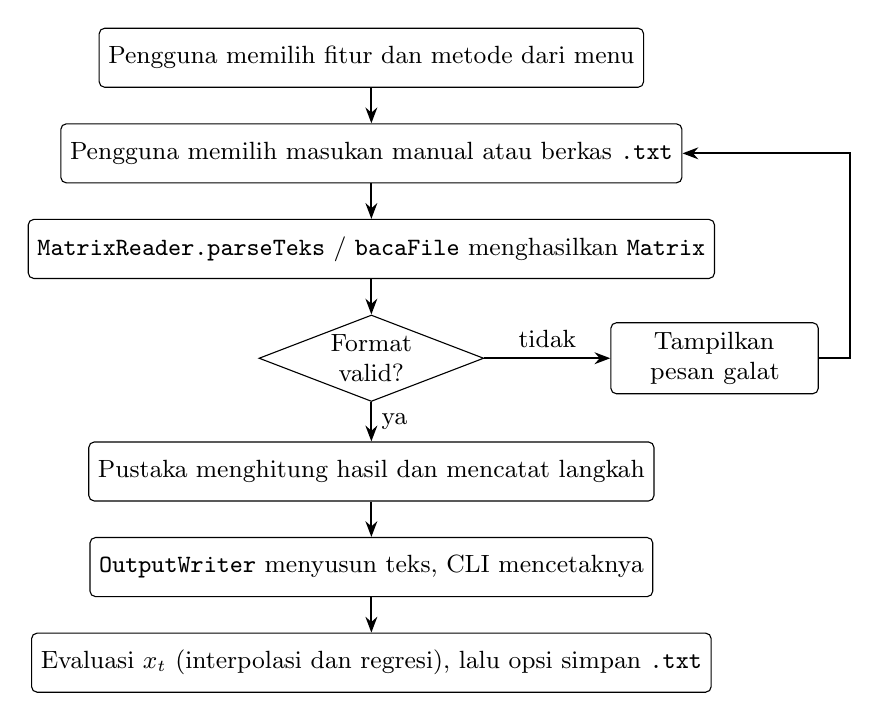
\begin{tikzpicture}[
  node distance=0.45cm,
  langkah/.style={draw, rounded corners=2pt, minimum width=6.6cm, minimum height=0.75cm, align=center, font=\small},
  pilih/.style={draw, diamond, aspect=2.6, align=center, font=\small, inner sep=1pt},
  panah/.style={-{Stealth[length=2mm]}, thick}
]
\node[langkah] (a) {Pengguna memilih fitur dan metode dari menu};
\node[langkah, below=of a] (b) {Pengguna memilih masukan manual atau berkas \texttt{.txt}};
\node[langkah, below=of b] (c) {\texttt{MatrixReader.parseTeks} / \texttt{bacaFile} menghasilkan \texttt{Matrix}};
\node[pilih, below=of c] (d) {Format\\valid?};
\node[langkah, below=0.5cm of d] (e) {Pustaka menghitung hasil dan mencatat langkah};
\node[langkah, below=of e] (f) {\texttt{OutputWriter} menyusun teks, CLI mencetaknya};
\node[langkah, below=of f] (g) {Evaluasi $x_t$ (interpolasi dan regresi), lalu opsi simpan \texttt{.txt}};
\node[langkah, right=1.6cm of d, minimum width=2.6cm, text width=2.4cm] (err) {Tampilkan pesan galat};
\draw[panah] (a) -- (b);
\draw[panah] (b) -- (c);
\draw[panah] (c) -- (d);
\draw[panah] (d) -- node[right, font=\small]{ya} (e);
\draw[panah] (d.east) -- node[above, font=\small]{tidak} (err.west);
\draw[panah] (err.east) -- ++(0.4,0) |- (b.east);
\draw[panah] (e) -- (f);
\draw[panah] (f) -- (g);
\end{tikzpicture}
\end{adjustbox}
\caption{Alur penggunaan satu fitur pada CLI}
\label{fig:alur}
\end{figure}

\subsubsection{Antarmuka Grafis (GUI)}

GUI dibuat dengan Java Swing. Kami memilih Swing karena sudah termasuk dalam JDK, sehingga \texttt{.jar} yang sama dapat dijalankan dengan \texttt{java -jar} tanpa pustaka tambahan. JavaFX sejak Java 11 terpisah dari JDK dan membutuhkan dependensi khusus sistem operasi.

\isi{Jelaskan struktur GUI yang sudah jadi (MainFrame dengan JTabbedPane berisi enam tab fitur, panel langkah dengan tombol sebelumnya/berikutnya, panel grafik kurva dengan Graphics2D, tombol buka berkas dan simpan hasil), lalu buat kotak kelas untuk setiap kelas GUI seperti di atas.}

\begin{figure}[H]
\centering
\gambarkosong{Tangkapan layar GUI (gambar/gui-utama.png)}{5cm}
\caption{Tampilan utama GUI}
\label{fig:gui}
\end{figure}

\subsection{Maven dan Pembuatan Berkas \texttt{.jar}}

Apache Maven mengatur kompilasi dan pengemasan program berdasarkan berkas \texttt{pom.xml}. Berkas ini menetapkan versi Java (\texttt{maven.compiler.release} = 17), \textit{encoding} UTF-8, dan plugin \texttt{maven-shade-plugin}. Plugin shade menggabungkan semua kelas ke dalam satu \texttt{.jar} dan menuliskan kelas utama \texttt{algeo.App} ke \textit{manifest}, sehingga berkas dapat dijalankan langsung.

\begin{lstlisting}
mvn clean package
cp target/profil2spartans-1.0-SNAPSHOT.jar bin/
java -jar bin/profil2spartans-1.0-SNAPSHOT.jar        # GUI
java -jar bin/profil2spartans-1.0-SNAPSHOT.jar cli    # CLI
\end{lstlisting}
\isi{Cocokkan nama berkas .jar dan argumen dengan README final.}

Perintah \texttt{mvn clean package} menghapus hasil kompilasi lama, mengompilasi seluruh kode di \texttt{src/main/java}, lalu mengemasnya ke folder \texttt{target}. Karena pustaka tidak bergantung pada dependensi luar, \texttt{.jar} yang dihasilkan juga dapat dipakai sebagai pustaka oleh program Java lain dengan menambahkannya ke \textit{classpath}.
\clearpage
\section{Eksperimen}

Bagian ini berisi hasil eksekusi program terhadap seluruh kasus uji pada Bab 5 spesifikasi. Berkas masukannya tersimpan di folder \texttt{test/} dengan pola nama \texttt{spl\_*.txt}, \texttt{det\_*.txt}, \texttt{inverse\_*.txt}, \texttt{interpolasi\_*.txt}, dan \texttt{regresi\_*.txt}. Angka pada bagian \textit{Output} adalah keluaran pustaka kelompok yang sudah dibulatkan ke 3 angka di belakang koma, sama seperti yang ditampilkan program. Sebagai pembanding, kami menghitung solusi eksak dengan aritmetika pecahan (\textit{rational}) di SymPy.

\subsection{Determinan Matriks}

Setiap kasus diuji dengan metode reduksi baris (OBE) dan ekspansi kofaktor.

\subsubsection{Kasus Uji 1}
\begin{kasus}
\ubag{Input}
\[
\begin{bmatrix}
0 & 2 & -1 & 3 \\
4 & 1 & 2 & -2 \\
-2 & 3 & 0 & 1 \\
1 & -1 & 5 & 2
\end{bmatrix}
\]
\ubag{Output}
\begin{center}
OBE: $\det(A) = -259$ \qquad Kofaktor: $\det(A) = -259$
\end{center}
\begin{center}
    \begin{minipage}{0.48\textwidth}
        \centering
        \tangkapan{det_1_obe}
    \end{minipage}\hfill
    \begin{minipage}{0.48\textwidth}
        \centering
        \tangkapan{det_1_kof}
    \end{minipage}
\end{center}
\end{kasus}

\subsubsection{Kasus Uji 2}
\begin{kasus}
\ubag{Input}
\[
\begin{bmatrix}
2 & -1 & 3 & 0 & 4 \\
1 & 2 & -2 & 5 & -1 \\
3 & 1 & 1 & 2 & 0 \\
4 & -1 & 3 & 2 & 0 \\
5 & 0 & 4 & 2 & 4
\end{bmatrix}
\]
\ubag{Output}
\begin{center}
OBE: $\det(A) = 0$ \qquad Kofaktor: $\det(A) = 0$
\end{center}
\begin{center}
    \begin{minipage}{0.48\textwidth}
        \centering
        \tangkapan{det_2_obe}
    \end{minipage}\hfill
    \begin{minipage}{0.48\textwidth}
        \centering
        \tangkapan{det_2_kof}
    \end{minipage}
\end{center}
\end{kasus}
\subsubsection{Kasus Uji 3}

\begin{kasus}
\ubag{Input}
\[
\begin{bmatrix}
1/2 & 1 & 0 & 1/2 \\
1/2 & 5/4 & 1/4 & 1/2 \\
-1/10 & -2/5 & 1/5 & -3/10 \\
3/5 & 5/4 & 9/20 & 3/5
\end{bmatrix}
\]
Program tidak menerima pecahan, sehingga berkas masukan
(\texttt{det\_5\_1\_3.txt}) ditulis dalam desimal ($0.5$, $1.25$, $0.25$,
$-0.1$, $-0.4$, $0.2$, $-0.3$, $0.6$, $0.45$).
\ubag{Output}
\begin{center}
OBE: $\det(A) = 0.01$ \qquad Kofaktor: $\det(A) = 0.01$ \qquad
Eksak: $1/100 = 0.01$
\end{center}
\begin{center}
    \begin{minipage}{0.48\textwidth}
        \centering
        \tangkapan{det_3_obe}
    \end{minipage}\hfill
    \begin{minipage}{0.48\textwidth}
        \centering
        \tangkapan{det_3_kof}
    \end{minipage}
\end{center}
\end{kasus}

\textbf{Analisis.} Kasus 1, 2, dan 3 semuanya menghasilkan nilai yang sama persis untuk kedua metode. Berdasarkan pengujian matriks 5x5, kedua metode sama-sama menghasilkan determinan 0 lalu algoritma Kofaktor bekerja  dengan menjadikan Baris 1 sebagai acuan untuk meng-skip minor bernilai nol sementara OBE mendeteksi elemen pivot nol di langkah ke-14 yang otomatis membuat perkalian diagonal utamanya mutlak bernilai 0.
 Keakuratan serupa juga terbukti pada matriks desimal pecahan 4x4 yang menghasilkan determinan 0.01. Kofaktor  mengoptimasi komputasi dengan memotong perhitungan pada elemen nol di Baris 1 sedangkan OBE berhasil mereduksi matriks menjadi segitiga atas dengan penyesuaian tanda kali -1 akibat operasi tukar baris sehingga hasil kali seluruh elemen diagonal utamanya secara konsisten berujung pada nilai 0.01 yang identik.

\subsection{Invers Matriks}

Setiap kasus diuji dengan metode augmentasi dan metode adjoin.

\subsubsection{Kasus Uji 1}
\begin{kasus}
\ubag{Input}
\[
\begin{bmatrix}
0 & 1 & 2 & -1 \\
1 & 0 & 1 & 2 \\
2 & 1 & 0 & 1 \\
-1 & 2 & 1 & 0
\end{bmatrix}
\]
\ubag{Output}
Augmentasi dan adjoin menghasilkan matriks yang sama:
\[
A^{-1} = \begin{bmatrix}
0.2 & -0.1 & 0.4 & -0.3 \\
-0.1 & -0.2 & 0.3 & 0.4 \\
0.4 & 0.3 & -0.2 & -0.1 \\
-0.3 & 0.4 & -0.1 & 0.2
\end{bmatrix}
\]
\textbf{Augmentasi}
\tangkapan{hasil_inverse_1_aug_1}
\tangkapan{hasil_inverse_1_aug_2}
\tangkapan{hasil_inverse_1_aug_3}
\tangkapan{hasil_inverse_1_aug_4}

\textbf{Kofaktor}
\tangkapan{hasil_inverse_1_kof_1}
\tangkapan{hasil_inverse_1_kof_2}
\tangkapan{hasil_inverse_1_kof_3}
\end{kasus}

\subsubsection{Kasus Uji 2}
\begin{kasus}
\ubag{Input}
\[
\begin{bmatrix}
1 & 2 & 0 & -1 & 3 \\
2 & -1 & 4 & 0 & 1 \\
0 & 3 & 1 & 2 & -2 \\
4 & 0 & 5 & 1 & 2 \\
3 & 1 & 4 & -1 & 4
\end{bmatrix}
\]
\ubag{Output}
Kedua metode: \texttt{matriks tidak memiliki balikan (Matriks singular, determinan = 0)}.

\textbf{Augmentasi}
\tangkapan{inverse_2_aug_1}
\tangkapan{inverse_2_aug_2}
\tangkapan{inverse_2_aug_3}
\tangkapan{inverse_2_aug_4}
\tangkapan{inverse_2_aug_5}
\tangkapan{inverse_2_aug_6}

\textbf{Kofaktor}
\tangkapan{inverse_2_kof_1}
\end{kasus}

\textbf{Analisis.} Pada kasus 1, kedua metode menghasilkan invers matriks yang sama. Hasil tersebut juga sesuai dengan nilai yang ditulis dalam bentuk nilai sebenarnya (tanpa pembulatan desimal), yaitu matriks dengan elemen-elemen yang merupakan kelipatan $1/10$. Selain itu, karena matriks $A$ simetris, maka matriks balikannya pun juga simetris.

Sementara, di kasus 2, matriks tidak memiliki invers matriks karena baris kelima merupakan hasil penjumlahan baris pertama dan baris kedua. Karena itu, baris-baris matriks tidak bebas secara linier dan $\det(A) = 0$. Pada metode augmentasi, kondisi ini baru terlihat ketika tidak ditemukan pivot yang dapat digunakan pada salah satu kolom. Sementara itu, metode adjoin terlebih dahulu memeriksa determinan. Karena determinannya nol, jadi proses mencari balikan dihentikan.

\subsection{Sistem Persamaan Linier $Ax = b$}

Setiap kasus dijalankan dengan keempat metode. Metode matriks balikan dan kaidah Cramer hanya bisa dipakai jika $A$ persegi dan $\det(A) \neq 0$ yang dimana jika syarat itu tidak terpenuhi, program menampilkan pesan alasannya.

\subsubsection{Kasus Uji 1}
\begin{kasus}
\ubag{Input}
\[
A = \begin{bmatrix}
0 & 2 & -1 & 1 \\
1 & -1 & 2 & 3 \\
2 & 1 & 1 & -1 \\
-1 & 3 & 0 & 2
\end{bmatrix}, \quad
b = \begin{bmatrix} -5 \\ 15 \\ 1 \\ -3 \end{bmatrix}
\]
\ubag{Output}
\begin{center}
Gauss, Gauss-Jordan, Balikan, Cramer: $x_1 = 1$, $x_2 = -2$, $x_3 = 3$, $x_4 = 2$
\end{center}
\textbf{Eliminasi Gauss}
\tangkapan{spl_1_gauss_1}
\tangkapan{spl_1_gauss_2}
\tangkapan{spl_1_gauss_3}

\textbf{Eliminasi Gauss-Jordan}
\tangkapan{spl_1_gj_1}
\tangkapan{spl_1_gj_2}
\tangkapan{spl_1_gj_3}

\textbf{Metode Matriks Balikan}
\tangkapan{spl_1_balikan_1}
\tangkapan{spl_1_balikan_2}
\tangkapan{spl_1_balikan_3}

\textbf{Kaidah Cramer}
\tangkapan{spl_1_cramer_1}
\end{kasus}

\subsubsection{Kasus Uji 2}
\begin{kasus}
\ubag{Input}
\[
A = \begin{bmatrix}
1 & 2 & -1 & 0 & 3 \\
2 & 4 & 1 & -1 & 5 \\
-1 & -2 & 2 & 3 & -1
\end{bmatrix}, \quad
b = \begin{bmatrix} 2 \\ 10 \\ -1 \end{bmatrix}
\]
\ubag{Output}
Gauss dan Gauss-Jordan (tak hingga solusi):
\begin{align*}
x_1 &= 3.9 - 2t_1 - 2.9t_2, & x_2 &= t_1, & x_3 &= 1.9 + 0.1t_2, \\
x_4 &= -0.3 - 0.7t_2, & x_5 &= t_2 .
\end{align*}
Balikan dan Cramer: \texttt{tidak bisa dipakai karena jumlah persamaan tidak sama dengan jumlah variabel}.
\textbf{Eliminasi Gauss}
\tangkapan{spl_2_gauss_1}
\tangkapan{spl_2_gauss_2}

\textbf{Eliminasi Gauss-Jordan}
\tangkapan{spl_2_gj_1}
\tangkapan{spl_2_gj_2}

\textbf{Metode Matriks Balikan}
\tangkapan{spl_2_balikan_1}

\textbf{Kaidah Cramer}
\tangkapan{spl_2_cramer_1}
\end{kasus}

\subsubsection{Kasus Uji 3}
\begin{kasus}
\ubag{Input}
\[
A = \begin{bmatrix}
1 & -2 & 3 & 1 \\
2 & 1 & -1 & 4 \\
0 & 3 & 2 & -2 \\
3 & -1 & 2 & 5
\end{bmatrix}, \quad
b = \begin{bmatrix} 4 \\ -1 \\ 3 \\ 4 \end{bmatrix}
\]
\ubag{Output}
Gauss dan Gauss-Jordan: \texttt{solusi tidak ada}.\\
Balikan dan Cramer: \texttt{tidak bisa dipakai karena det(A) = 0}.
\textbf{Eliminasi Gauss}
\tangkapan{spl_3_gauss_1}
\tangkapan{spl_3_gauss_2}

\textbf{Eliminasi Gauss-Jordan}
\tangkapan{spl_3_gj_1}
\tangkapan{spl_3_gj_2}
\tangkapan{spl_3_gj_3}

\textbf{Metode Matriks Balikan}
\tangkapan{spl_3_balikan_1}

\textbf{Kaidah Cramer}
\tangkapan{spl_3_cramer_1}
\end{kasus}

\subsubsection{Kasus Uji 4: Matriks \textit{Discrete Laplacian}}
\begin{kasus}
\ubag{Input}
$A_n$ bernilai 2 pada diagonal, $-1$ tepat di atas dan di bawah diagonal, dan 0 di tempat lain dan $b$ berisi angka 1. Diuji untuk $n = 6$ dan $n = 10$.
\ubag{Output}
\begin{center}
\begin{tabular}{lcccccccccc}
\toprule
$n$ & $x_1$ & $x_2$ & $x_3$ & $x_4$ & $x_5$ & $x_6$ & $x_7$ & $x_8$ & $x_9$ & $x_{10}$ \\
\midrule
6  & 3 & 5 & 6 & 6 & 5 & 3 & & & & \\
10 & 5 & 9 & 12 & 14 & 15 & 15 & 14 & 12 & 9 & 5 \\
\bottomrule
\end{tabular}
\end{center}
Keempat metode memberi hasil yang sama setelah pembulatan.
\textbf{\boldmath$n = 6$}

\textbf{Eliminasi Gauss}
\tangkapan{spl_4_n6_gauss_1}
\tangkapan{spl_4_n6_gauss_2}
\tangkapan{spl_4_n6_gauss_3}

\textbf{Eliminasi Gauss-Jordan}
\tangkapan{spl_4_n6_gj_1}
\tangkapan{spl_4_n6_gj_2}
\tangkapan{spl_4_n6_gj_3}
\tangkapan{spl_4_n6_gj_4}
\tangkapan{spl_4_n6_gj_5}

\textbf{Metode Matriks Balikan}
\tangkapan{spl_4_n6_balikan_1}
\tangkapan{spl_4_n6_balikan_2}
\tangkapan{spl_4_n6_balikan_3}
\tangkapan{spl_4_n6_balikan_4}
\tangkapan{spl_4_n6_balikan_5}
\tangkapan{spl_4_n6_balikan_6}

\textbf{Kaidah Cramer}
\tangkapan{spl_4_n6_cramer_1}
\tangkapan{spl_4_n6_cramer_2}

\textbf{\boldmath$n = 10$}

\textbf{Eliminasi Gauss}
\tangkapan{spl_4_n10_gauss_1}
\tangkapan{spl_4_n10_gauss_2}
\tangkapan{spl_4_n10_gauss_3}
\tangkapan{spl_4_n10_gauss_4}
\tangkapan{spl_4_n10_gauss_5}
\tangkapan{spl_4_n10_gauss_6}

\textbf{Eliminasi Gauss-Jordan}
\tangkapan{spl_4_n10_gj_1}
\tangkapan{spl_4_n10_gj_2}
\tangkapan{spl_4_n10_gj_3}
\tangkapan{spl_4_n10_gj_4}
\tangkapan{spl_4_n10_gj_5}
\tangkapan{spl_4_n10_gj_6}
\tangkapan{spl_4_n10_gj_7}
\tangkapan{spl_4_n10_gj_8}
\tangkapan{spl_4_n10_gj_9}
\tangkapan{spl_4_n10_gj_10}
\tangkapan{spl_4_n10_gj_11}
\tangkapan{spl_4_n10_gj_12}
\tangkapan{spl_4_n10_gj_13}
\tangkapan{spl_4_n10_gj_14}
\tangkapan{spl_4_n10_gj_15}
\tangkapan{spl_4_n10_gj_16}
\tangkapan{spl_4_n10_gj_17}

\textbf{Metode Matriks Balikan}
\tangkapan{spl_4_n10_balikan_1}
\tangkapan{spl_4_n10_balikan_2}
\tangkapan{spl_4_n10_balikan_3}
\tangkapan{spl_4_n10_balikan_4}
\tangkapan{spl_4_n10_balikan_5}
\tangkapan{spl_4_n10_balikan_6}
\tangkapan{spl_4_n10_balikan_7}
\tangkapan{spl_4_n10_balikan_8}
\tangkapan{spl_4_n10_balikan_9}
\tangkapan{spl_4_n10_balikan_10}
\tangkapan{spl_4_n10_balikan_11}
\tangkapan{spl_4_n10_balikan_12}
\tangkapan{spl_4_n10_balikan_13}
\tangkapan{spl_4_n10_balikan_14}
\tangkapan{spl_4_n10_balikan_15}
\tangkapan{spl_4_n10_balikan_16}
\tangkapan{spl_4_n10_balikan_17}
\tangkapan{spl_4_n10_balikan_18}

\textbf{Kaidah Cramer}
\tangkapan{spl_4_n10_cramer_1}
\tangkapan{spl_4_n10_cramer_2}
\tangkapan{spl_4_n10_cramer_3}
\tangkapan{spl_4_n10_cramer_4}
\end{kasus}

\textbf{Analisis.} Pada kasus 1, keempat metode memberikan jawaban yang sama dengan solusi eksak. Jika dilihat sebelum dibulatkan, nilainya sedikit berbeda antarmetode. Contohnya, $x_1$ bernilai $1.0000000000000002$ pada eliminasi Gauss dan $1.0000000000000004$ pada Gauss-Jordan. Perbedaan ini baru muncul di digit ke-16, sesuai dengan batas ketelitian \texttt{double}, dan hilang setelah dibulatkan ke 3 angka di belakang koma.

Kasus 2 hanya memiliki 3 persamaan untuk 5 variabel, jadi paling sedikit ada 2 variabel bebas. Program memilih $x_2$ dan $x_5$ sebagai parameter karena kolom keduanya tidak mendapat pivot. Kami membandingkannya dengan hasil SymPy dan bentuknya sama: $x_1 = 39/10 - 2x_2 - 29x_5/10$, $x_3 = 19/10 + x_5/10$, dan $x_4 = -3/10 - 7x_5/10$. Metode balikan dan Cramer langsung ditolak karena matriks $A$ tidak persegi.

Pada kasus 3, $\operatorname{rank}(A) = 3$, sedangkan $\operatorname{rank}([A\,|\,b]) = 4$. Akibatnya, setelah eliminasi muncul baris $0 = c$ dengan $c \neq 0$ sehingga SPL tidak memiliki solusi. Metode balikan dan Cramer sudah berhenti lebih awal karena $\det(A) = 0$, tetapi pesan itu belum menjelaskan apakah SPL-nya tidak punya solusi atau punya banyak solusi. Untuk kasus seperti ini, hanya eliminasi Gauss dan Gauss-Jordan yang memberikan jawaban lengkap.

Kasus 4 kami pakai untuk melihat kestabilan numerik keempat metode. Solusi eksaknya mengikuti rumus $x_i = i(n+1-i)/2$, dan hasil program untuk $n = 6$ maupun $n = 10$ cocok dengan rumus tersebut. Matriks Laplacian bersifat dominan diagonal sehingga \textit{partial pivoting} tidak perlu menukar baris serta pada tangkapan layar, jumlah tukar baris tercatat 0. Galat terbesar sebelum pembulatan muncul pada kaidah Cramer untuk $n = 10$, misalnya $x_2 = 9.000000000000004$. Hal ini masuk akal karena Cramer menghitung 11 determinan secara terpisah dan setiap determinan membawa galat pembulatannya sendiri.

\subsection{SPL Berbentuk Matriks \textit{Augmented}}

\subsubsection{Kasus Uji 1}
\begin{kasus}
\ubag{Input}
\[
\left[\begin{array}{cccc|c}
0 & 1 & -1 & 2 & -1 \\
2 & 0 & 1 & -1 & 3 \\
-1 & 2 & 0 & 1 & -3 \\
1 & -1 & 2 & 0 & 9
\end{array}\right]
\]
\ubag{Output}
\begin{center}
Keempat metode: $x_1 = 1$, $x_2 = -2$, $x_3 = 3$, $x_4 = 2$
\end{center}
\textbf{Eliminasi Gauss}
\tangkapan{spl_aug_1_gauss_1}
\tangkapan{spl_aug_1_gauss_2}
\tangkapan{spl_aug_1_gauss_3}

\textbf{Eliminasi Gauss-Jordan}
\tangkapan{spl_aug_1_gj_1}
\tangkapan{spl_aug_1_gj_2}
\tangkapan{spl_aug_1_gj_3}

\textbf{Metode Matriks Balikan}
\tangkapan{spl_aug_1_balikan_1}
\tangkapan{spl_aug_1_balikan_2}
\tangkapan{spl_aug_1_balikan_3}

\textbf{Kaidah Cramer}
\tangkapan{spl_aug_1_cramer_1}
\end{kasus}

\subsubsection{Kasus Uji 2}
\begin{kasus}
\ubag{Input}
\[
\left[\begin{array}{cccccc|c}
1 & 0 & 2 & -1 & 0 & 3 & -7 \\
0 & 1 & -1 & 2 & 1 & 0 & 6 \\
2 & -1 & 0 & 1 & 3 & -2 & 13 \\
1 & 1 & 1 & 1 & 1 & 1 & 3
\end{array}\right]
\]
\ubag{Output}
Gauss dan Gauss-Jordan (tak hingga solusi):
\begin{align*}
x_1 &= 5.8 - t_1 - 1.6t_2, & x_2 &= 2.6 - t_1 - 0.2t_2, & x_3 &= -3.4 + t_1 + 0.8t_2, \\
x_4 &= t_1, & x_5 &= t_2, & x_6 &= -2 .
\end{align*}
Balikan dan Cramer: tidak dapat dipakai karena matriks koefisien berukuran $4 \times 6$.
\textbf{Eliminasi Gauss}
\tangkapan{spl_aug_2_gauss_1}
\tangkapan{spl_aug_2_gauss_2}

\textbf{Eliminasi Gauss-Jordan}
\tangkapan{spl_aug_2_gj_1}
\tangkapan{spl_aug_2_gj_2}
\tangkapan{spl_aug_2_gj_3}

\textbf{Metode Matriks Balikan}
\tangkapan{spl_aug_2_balikan_1}

\textbf{Kaidah Cramer}
\tangkapan{spl_aug_2_cramer_1}
\end{kasus}

\textbf{Analisis.} Elemen $a_{11}$ pada kasus 1 bernilai 0. Tanpa pertukaran baris, langkah pertama eliminasi akan membagi dengan nol. Dengan \textit{partial pivoting}, program menukar baris 1 dan baris 2 karena nilai mutlak terbesar pada kolom pertama adalah 2, lalu eliminasi berjalan seperti biasa. Solusinya, $(1, -2, 3, 2)$, kebetulan sama dengan solusi SPL kasus 1 pada subbab sebelumnya.

Matriks koefisien pada kasus 2 berukuran $4 \times 6$ sehingga balikan dan Cramer tidak bisa dipakai. Hasil eliminasi memberikan dua variabel bebas, yaitu $x_4$ dan $x_5$. Yang perlu diperhatikan, $x_6$ tetap bernilai $-2$ berapa pun nilai parameternya, artinya setiap solusi SPL ini memenuhi $x_6 = -2$. Hasil ini cocok dengan perhitungan eksak.

\subsection{SPL Berbentuk Umum}

\subsubsection{Kasus Uji 1}
\begin{kasus}
\ubag{Input}
\[
\begin{cases}
3x_1 + 2x_2 - x_3 + 4x_4 = 5 \\
x_1 - 3x_2 + 2x_3 + x_4 = -2 \\
4x_1 + x_2 + 5x_3 - 2x_4 = 7 \\
2x_1 - x_2 + 3x_3 + x_4 = 3
\end{cases}
\]
\ubag{Output}
\begin{center}
\begin{tabular}{lcccc}
\toprule
 & $x_1$ & $x_2$ & $x_3$ & $x_4$ \\
\midrule
Program (4 metode) & $-0.114$ & $1.841$ & $1.432$ & $0.773$ \\
Nilai eksak & $-5/44$ & $81/44$ & $63/44$ & $17/22$ \\
\bottomrule
\end{tabular}
\end{center}
\textbf{Eliminasi Gauss}
\tangkapan{spl_umum_1_gauss_1}
\tangkapan{spl_umum_1_gauss_2}

\textbf{Eliminasi Gauss-Jordan}
\tangkapan{spl_umum_1_gj_1}
\tangkapan{spl_umum_1_gj_2}
\tangkapan{spl_umum_1_gj_3}

\textbf{Metode Matriks Balikan}
\tangkapan{spl_umum_1_balikan_1}
\tangkapan{spl_umum_1_balikan_2}
\tangkapan{spl_umum_1_balikan_3}

\textbf{Kaidah Cramer}
\tangkapan{spl_umum_1_cramer_1}
\end{kasus}

\subsubsection{Kasus Uji 2}
\begin{kasus}
\ubag{Input}
Sistem 9 persamaan dan 9 variabel pada spesifikasi 5.5.2, ditulis sebagai matriks \textit{augmented} $9 \times 10$ dengan mengelompokkan koefisien setiap variabel. Contohnya, persamaan keempat menjadi $0.03521x_1 + 0.68x_2 + 0.03521x_4 + 0.68x_6 + 0.03521x_7 + 0.55432x_9 = 8.47$.
\ubag{Output}
Gauss dan Gauss-Jordan (tak hingga solusi, satu parameter):
\begin{align*}
x_1 &= 5.776 - 0.462t, & x_2 &= 4.464 - 0.387t, & x_3 &= -0.24 + 0.849t, \\
x_4 &= -0.736 + 0.971t, & x_5 &= 5.224 - 0.538t, & x_6 &= 7.512 - 0.433t, \\
x_7 &= 4.227 - 0.416t, & x_8 &= 4.773 - 0.584t, & x_9 &= t .
\end{align*}
Balikan dan Cramer: \texttt{tidak bisa dipakai karena det(A) = 0}.
\textbf{Eliminasi Gauss}
\tangkapan{spl_umum_2_gauss_1}
\tangkapan{spl_umum_2_gauss_2}
\tangkapan{spl_umum_2_gauss_3}
\tangkapan{spl_umum_2_gauss_4}
\tangkapan{spl_umum_2_gauss_5}
\tangkapan{spl_umum_2_gauss_6}
\tangkapan{spl_umum_2_gauss_7}
\tangkapan{spl_umum_2_gauss_8}
\tangkapan{spl_umum_2_gauss_9}
\tangkapan{spl_umum_2_gauss_10}

\textbf{Eliminasi Gauss-Jordan}
\tangkapan{spl_umum_2_gj_1}
\tangkapan{spl_umum_2_gj_2}
\tangkapan{spl_umum_2_gj_3}
\tangkapan{spl_umum_2_gj_4}
\tangkapan{spl_umum_2_gj_5}
\tangkapan{spl_umum_2_gj_6}
\tangkapan{spl_umum_2_gj_7}
\tangkapan{spl_umum_2_gj_8}
\tangkapan{spl_umum_2_gj_9}
\tangkapan{spl_umum_2_gj_10}
\tangkapan{spl_umum_2_gj_11}
\tangkapan{spl_umum_2_gj_12}
\tangkapan{spl_umum_2_gj_13}
\tangkapan{spl_umum_2_gj_14}
\tangkapan{spl_umum_2_gj_15}

\textbf{Metode Matriks Balikan}
\tangkapan{spl_umum_2_balikan_1}

\textbf{Kaidah Cramer}
\tangkapan{spl_umum_2_cramer_1}
\end{kasus}

\textbf{Analisis.} Kasus 1 memiliki solusi tunggal dan keempat metode memberikan hasil yang sama. Nilai eksaknya berupa pecahan berpenyebut 44 (misalnya $x_1 = -5/44$) sehingga program hanya bisa menampilkannya sebagai desimal yang dibulatkan.

Kasus 2 awalnya terlihat seperti SPL persegi biasa dengan 9 persamaan dan 9 variabel. Namun, perhitungan eksak dengan pecahan menunjukkan $\operatorname{rank}(A) = \operatorname{rank}([A\,|\,b]) = 8$ dan $\det(A) = 0$, jadi jawaban solusi tak terhingga memang benar. Penyebabnya cukup mudah dilihat. Jika persamaan 1, 2, dan 3 dijumlahkan, ruas kirinya menjadi $x_1 + x_2 + \dots + x_9$, dan hal yang sama terjadi jika persamaan 7, 8, dan 9 dijumlahkan. Ruas kanannya pun sama, yaitu $10 + 12 + 9 = 31$ dan $11 + 8.5 + 11.5 = 31$. Dengan kata lain, salah satu persamaan merupakan kombinasi linier dari persamaan lain, tetapi SPL-nya tetap konsisten.

Kasus ini juga menguji toleransi nol pada program. Dalam \textit{floating point}, eliminasi tidak selalu menghasilkan nol yang tepat tetapi yang tersisa bisa berupa galat pembulatan yang sangat kecil. Jika batas nol terlalu ketat, sisa tersebut dapat dianggap sebagai pivot yang sah dan program akan melaporkan solusi tunggal yang keliru. Dengan toleransi relatif dari kelas \texttt{Toleransi}, kolom $x_9$ dikenali tidak memiliki pivot sehingga $x_9$ menjadi parameter $t$.

\subsection{Aplikasi Sistem Persamaan Linier}

\begin{kasus}
\ubag{Input}
Data luas rumah dan harga: $(1, 3)$, $(2, 5)$, $(3, 6)$. Dengan $\sum x_i = 6$, $\sum x_i^2 = 14$, $\sum y_i = 14$, dan $\sum x_i y_i = 31$, persamaan normalnya
\[
\left[\begin{array}{cc|c}
3 & 6 & 14 \\
6 & 14 & 31
\end{array}\right].
\]
\ubag{Output}
\begin{center}
Keempat metode: $\theta_0 = 1.667$, $\theta_1 = 1.5$, sehingga $y = 1.667 + 1.5x$.
\end{center}
\textbf{Eliminasi Gauss}
\tangkapan{spl_aplikasi_gauss_1}

\textbf{Eliminasi Gauss-Jordan}
\tangkapan{spl_aplikasi_gj_1}

\textbf{Metode Matriks Balikan}
\tangkapan{spl_aplikasi_balikan_1}

\textbf{Kaidah Cramer}
\tangkapan{spl_aplikasi_cramer_1}
\end{kasus}

\textbf{Analisis.} Nilai eksaknya adalah $\theta_0 = 5/3$ dan $\theta_1 = 3/2$. Garis $y = 1.667 + 1.5x$ tidak melewati ketiga titik secara tepat dan pada $x = 2$, model memprediksi $4.667$, sedangkan datanya bernilai 5. Hal ini wajar karena ketiga titik memang tidak segaris. Persamaan normal tidak mencari garis yang melewati semua titik, tetapi garis dengan jumlah kuadrat galat paling kecil. Ide yang sama kami pakai lagi pada regresi \textit{spline}, hanya saja jumlah basisnya lebih banyak.

\subsection{Studi Kasus Interpolasi Polinomial}

\subsubsection{Studi Kasus 1}
\begin{kasus}
\ubag{Input}
\begin{center}
\begin{tabular}{c|ccccccc}
$x$ & 0.2 & 0.4 & 0.6 & 0.8 & 1.0 & 1.2 & 1.4 \\ \hline
$f(x)$ & 0.182 & 0.336 & 0.470 & 0.588 & 0.693 & 0.788 & 0.875
\end{tabular}
\end{center}
Evaluasi di $x = 0.3$, $0.55$, $0.95$, dan $1.38$.
\ubag{Output}
\[
P(x) = 1.003x - 0.546x^2 + 0.479x^3 - 0.408x^4 + 0.208x^5 - 0.043x^6
\]
\begin{center}
\begin{tabular}{cccc}
\toprule
$x$ & $P(x)$ program & $\ln(1+x)$ & Selisih \\
\midrule
0.3  & 0.262 & 0.262 & $5.1 \times 10^{-4}$ \\
0.55 & 0.438 & 0.438 & $1.3 \times 10^{-4}$ \\
0.95 & 0.668 & 0.668 & $2.7 \times 10^{-5}$ \\
1.38 & 0.867 & 0.867 & $4.3 \times 10^{-4}$ \\
\bottomrule
\end{tabular}
\end{center}
\begin{center}
    \begin{minipage}{0.48\textwidth}
        \centering
        \tangkapan{interpol1}
    \end{minipage}\hfill
    \begin{minipage}{0.48\textwidth}
        \centering
        \tangkapan{interpol1_eval}
    \end{minipage}
\end{center}\end{kasus}

\textbf{Analisis.} Koefisien konstanta yang dihitung program bernilai $6.8 \times 10^{-13}$, sehingga tampil sebagai 0. Nilai pada tabel data cocok dengan $\ln(1+x)$ yang dibulatkan ke 3 desimal (misalnya $\ln 1.2 = 0.18232$), sehingga kami memakai $\ln(1+x)$ sebagai pembanding meskipun spesifikasi tidak menyebutkan fungsi asalnya. Selisihnya selalu di bawah $10^{-3}$ dan sebagian besar berasal dari pembulatan data masukan. Selisih terbesar muncul di $x = 0.3$ dan $x = 1.38$, di dekat ujung domain, sesuai dengan teori bahwa polinomial derajat tinggi paling tidak akurat di dekat ujung interval.

\subsubsection{Studi Kasus 2: Suhu Komponen}
\begin{kasus}
\ubag{Input}
\begin{center}
\begin{tabular}{c|cccccc}
$t$ (menit) & 0 & 2 & 4 & 6 & 8 & 10 \\ \hline
$T$ ($^\circ$C) & 25.0 & 31.2 & 38.6 & 47.5 & 58.1 & 70.8
\end{tabular}
\end{center}
Evaluasi di $t = 1$, $3.5$, $7$, dan $9.2$, serta cari waktu saat $T = 65^\circ$C.
\ubag{Output}
\[
T(t) = 25 + 2.8925t + 0.069792t^2 + 0.020313t^3 - 0.0018229t^4 + 0.000078125t^5
\]
\begin{center}
\begin{tabular}{cccc}
\toprule
$t = 1$ & $t = 3.5$ & $t = 7$ & $t = 9.2$ \\
\midrule
$27.981$ & $36.617$ & $52.571$ & $65.425$ \\
\bottomrule
\end{tabular}
\end{center}
Komponen mencapai $65^\circ$C pada $t \approx 9.14$ menit.
\begin{center}
    \begin{minipage}{0.48\textwidth}
        \centering
        \tangkapan{interpol2}
    \end{minipage}\hfill
    \begin{minipage}{0.48\textwidth}
        \centering
        \tangkapan{interpol2_eval1}
    \end{minipage}\hfill
    \begin{minipage}{0.48\textwidth}
        \centering
        \tangkapan{interpol2_eval2}
    \end{minipage}
\end{center}
\end{kasus}

\textbf{Analisis.} Berdasarkan pengujian, program berhasil memproses enam titik data awal yang menghasilkan persamaan polinomial $P(x) = 25 + 2.893x + 0.07x^2 + 0.02x^3 - 0.002x^4$. Persamaan  tersebut digunakan  untuk memprediksi peningkatan suhu secara maju menghasilkan taksiran berurutan sebesar $27.981^\circ\text{C}$ pada menit ke-1, $36.617^\circ\text{C}$ pada menit ke-3.5, $52.571^\circ\text{C}$ pada menit ke-7, dan $65.425^\circ\text{C}$ pada menit ke-9.2. Sementara itu, untuk memecahkan persoalan waktu kerusakan komponen pada suhu spesifik $65^\circ\text{C}$  program  menukar variabel suhu menjadi sumbu $x$ dan waktu menjadi sumbu $y$. Melalui pendekatan tersebut, terbentuk persamaan balikan baru $P(x) = -12.719 + 0.702x - 0.009x^2$ yang saat dievaluasi pada target $P(65)$ menunjukkan bahwa komponen akan rusak pada menit ke-9.14.

\subsection{Studi Kasus Interpolasi \textit{Natural Cubic Spline}}

\begin{kasus}
\ubag{Input}
\begin{center}
\begin{tabular}{c|ccccc}
$x_i$ & 1 & 2 & 3 & 4 & 5 \\ \hline
$y_i$ & 2 & 3 & 4 & 5 & 6
\end{tabular}
\end{center}
\ubag{Output}
Turunan kedua: $M_0 = M_1 = M_2 = M_3 = M_4 = 0$.
\begin{align*}
S_0(x) &= 2 + (x - 1), & 1 \le x \le 2, \\
S_1(x) &= 3 + (x - 2), & 2 \le x \le 3, \\
S_2(x) &= 4 + (x - 3), & 3 \le x \le 4, \\
S_3(x) &= 5 + (x - 4), & 4 \le x \le 5 .
\end{align*}
Contoh evaluasi: $S(2.5) = 3.5$.

\tangkapan{ncs_1}
\tangkapan{ncs_2}
\tangkapan{ncs_3}
\tangkapan{ncs_4}
\tangkapan{ncs_5}
\tangkapan{ncs_6}
\tangkapan{ncs_7}
\tangkapan{ncs_8}
\tangkapan{ncs_9}
\tangkapan{ncs_10}
\tangkapan{ncs_11}
\tangkapan{ncs_12}
\tangkapan{ncs_13}
\tangkapan{ncs_14}
\tangkapan{ncs_15}
\tangkapan{ncs_16}
\tangkapan{ncs_17}
\end{kasus}

\textbf{Analisis.} Data titik-titik pada kasus ini membentuk garis lurus $y = x + 1$. 
Hasil interpolasi menunjukkan bahwa seluruh turunan kedua bernilai nol, 
sehingga setiap segmen spline juga berbentuk garis lurus. 
Dengan demikian, keempat segmen menghasilkan fungsi yang sama, yaitu 
$y = x + 1$. Contohnya, pada $x = 2.5$ diperoleh $S(2.5) = 3.5$.

\subsection{Studi Kasus Regresi Spline}

\begin{kasus}
\ubag{Input}
\begin{center}
\begin{tabular}{c|ccccccc}
$i$   & 0 & 1 & 2 & 3 & 4 & 5 & 6 \\ \hline
$x_i$ & $-3$ & $-2$ & $-1$ & 0 & 1 & 2 & 3 \\
$y_i$ & 19.9 & 4.4 & $-0.5$ & 2 & 6.5 & 15.6 & 38.1
\end{tabular}
\end{center}
Spline kubik ($d = 3$) dengan satu knot internal $\xi_1 = 0$, sehingga jumlah basisnya $M = 3 + 1 + 1 = 5$ untuk $N = 7$ titik data. Basis yang dipakai adalah $1, x, x^2, x^3, (x - 0)_+^3$.
\ubag{Output}
\[
\hat y(x) = 2 + 3x - x^3 + 2(x)_+^3
\quad\Longleftrightarrow\quad
\hat y(x) =
\begin{cases}
2 + 3x - x^3, & x \le 0,\\
2 + 3x + x^3, & x > 0.
\end{cases}
\]
\begin{center}
\begin{tabular}{c|ccccccc}
$x_i$ & $-3$ & $-2$ & $-1$ & 0 & 1 & 2 & 3 \\ \hline
$y_i$ & 19.9 & 4.4 & $-0.5$ & 2 & 6.5 & 15.6 & 38.1 \\
$\hat y(x_i)$ & 20 & 4 & 0 & 2 & 6 & 16 & 38 \\
$e_i = y_i - \hat y(x_i)$ & $-0.1$ & $0.4$ & $-0.5$ & $0$ & $0.5$ & $-0.4$ & $0.1$
\end{tabular}
\end{center}
Jumlah kuadrat galat $\sum e_i^2 = 0.84$. Contoh evaluasi: $\hat y(-2.5) = 10.125$, $\hat y(0.5) = 3.625$, $\hat y(1.5) = 9.875$.
\tangkapan{regresi_1}
\tangkapan{regresi_2}
\tangkapan{regresi_3}
\tangkapan{regresi_4}
\tangkapan{regresi_5}
\tangkapan{regresi_6}
\tangkapan{regresi_7}
\tangkapan{regresi_8}
\end{kasus}

\textbf{Analisis.} Program membentuk matriks desain $X$ berukuran $7 \times 5$, lalu menyelesaikan persamaan normal dengan eliminasi Gauss. Sebelum itu, $x$ diubah menjadi $u = x/3$ karena data berada di $[-3, 3]$ (titik tengahnya 0 dan setengah lebarnya 3). Koefisien yang diperoleh dalam $u$ adalah $b = (2,\ 9,\ 0,\ -27,\ 54)$. Setelah dikembalikan ke $x$, yaitu dengan membagi $b_j$ dengan $3^j$ untuk suku polinom dan membagi $b_4$ dengan $3^3$ untuk suku \textit{knot}, didapat $\beta = (2,\ 3,\ 0,\ -1,\ 2)$. Untuk memastikannya, kami juga menyelesaikan persamaan normal dalam $x$ secara eksak dengan pecahan:
\[
X^TX =
\begin{bmatrix}
7 & 0 & 28 & 0 & 36\\
0 & 28 & 0 & 196 & 98\\
28 & 0 & 196 & 0 & 276\\
0 & 196 & 0 & 1588 & 794\\
36 & 98 & 276 & 794 & 794
\end{bmatrix},
\qquad
X^Ty =
\begin{bmatrix} 86\\ 84\\ 608\\ 588\\ 1160 \end{bmatrix},
\]
dan hasilnya sama persis.

Koefisien $\beta_4 = 2$ mengubah koefisien $x^3$ dari $-1$ di kiri \textit{knot} menjadi $-1 + 2 = 1$ di kanan \textit{knot}. Kedua potongan kurva tetap tersambung mulus di $x = 0$ karena nilainya sama-sama 2, turunan pertamanya ($3 - 3x^2$ dan $3 + 3x^2$) sama-sama 3, dan turunan keduanya ($-6x$ dan $6x$) sama-sama 0. Perubahan koefisien kubik inilah yang membuat bentuk kurva di kiri dan kanan \textit{knot} berbeda. Di sisi kiri, $\hat y$ turun dari sekitar 20 ke 0, lalu naik lagi, sedangkan di sisi kanan, $\hat y$ naik makin curam sampai 38.

Karena $N = 7$ lebih besar daripada $M = 5$, kurva tidak harus melewati semua titik. Galat terbesarnya hanya $0.5$, yaitu di $x = -1$ dan $x = 1$. Polanya juga simetris dengan tanda berlawanan, $e(-x) = -e(x)$, sehingga model tidak cenderung terlalu tinggi di satu sisi saja. Jumlah kuadrat galatnya $0.84$, sangat kecil dibandingkan dengan total variasi data yang sekitar $1100$yang dimana artinya, model menjelaskan lebih dari $99.9\%$ variasi $y$. Kami menduga data ini dibuat dari kurva $2 + 3x \mp x^3$ yang diberi sedikit gangguan, dan regresi berhasil mendapatkan kembali koefisien kurva tersebut.

\clearpage
\section{Penutup}

\subsection{Kesimpulan}

Kami berhasil membangun pustaka aljabar linier dalam Java tanpa pustaka matematika eksternal. Pustaka ini mencakup empat metode SPL, dua metode determinan, dua metode matriks balikan, interpolasi polinomial, \textit{natural cubic spline}, dan regresi spline. Semua kasus uji pada spesifikasi menghasilkan jawaban yang sesuai dengan perhitungan eksak, termasuk kasus yang tidak memiliki solusi, kasus dengan tak hingga solusi, dan matriks singular.

Kelebihan sistem yang kami bangun:
\begin{itemize}[nosep]
  \item fitur lanjutan memakai ulang solver yang sama (spline memakai Gauss-Jordan, regresi memakai eliminasi Gauss, interpolasi memakai augmentasi) sehingga perbaikan pada satu solver langsung dirasakan semua fitur;
  \item toleransi nol yang relatif terhadap skala matriks yang membuat kasus hampir singular seperti SPL 9 variabel tetap terdeteksi dengan benar;
  \item determinan pada kaidah Cramer disimpan sebagai mantisa dan eksponen agar tidak \textit{overflow} pada matriks besar;
  \item masukan manual dan berkas melewati parser yang sama, begitu pula CLI dan GUI memakai penyusun teks hasil yang sama sehingga hasilnya konsisten.
\end{itemize}

Kekurangan yang kami sadari:
\begin{itemize}[nosep]
  \item \texttt{OBE}, \texttt{Kofaktor}, dan \texttt{Augmentasi} masih memakai toleransi tetap $10^{-12}$, belum toleransi relatif seperti solver SPL;
  \item pembulatan tampilan ke 3 desimal dapat membuat dua metode yang sama-sama benar terlihat berbeda, seperti determinan kasus uji 3 ($14.852$ dan $14.853$);
  \item interpolasi polinomial membentuk balikan matriks Vandermonde secara eksplisit, padahal matriks ini mudah menjadi \textit{ill-conditioned};
  \item SPL tridiagonal pada spline diselesaikan dengan Gauss-Jordan umum berkompleksitas $O(n^3)$, bukan algoritma khusus tridiagonal. Dengan batas 10 titik, hal ini belum berpengaruh pada kecepatan;
  \item ekspansi kofaktor dan metode adjoin dibatasi ukurannya karena kompleksitasnya terlalu besar.
\end{itemize}

\subsection{Saran}

Toleransi pada kelas determinan dan balikan sebaiknya diseragamkan dengan kelas \texttt{Toleransi}, agar semua metode memutuskan ``nol'' dengan cara yang sama. Untuk interpolasi, koefisien dapat dicari dengan menyelesaikan $Va = y$ langsung memakai eliminasi Gauss dengan \textit{partial pivoting}, tanpa membentuk $V^{-1}$, atau diganti dengan bentuk Newton yang tidak memerlukan matriks Vandermonde. SPL tridiagonal pada spline dapat diselesaikan dengan algoritma Thomas yang berkompleksitas $O(n)$ jika batas jumlah titik ingin dinaikkan. Untuk masalah pembulatan tampilan, program dapat menambahkan opsi untuk menampilkan lebih banyak digit ketika pengguna ingin membandingkan metode.

\subsection{Refleksi Anggota}

\isi{Setiap anggota menulis satu atau dua paragraf dengan kata-kata sendiri: bagian yang dikerjakan, kendala yang dihadapi, dan hal baru yang dipelajari. Contoh kendala nyata dari riwayat commit kelompok: determinan yang overflow, metode adjoin yang kehabisan memori, toleransi yang diganti menjadi relatif, dan normalisasi x pada regresi.}

\begin{komentar}{Refleksi 5.3.1: Neysa Alya Mukhbita}
kapan lagi whimsymaxxing di algeo (makasih lewi udah mau nurutin kemauan ney n kate) :3 so far seru banget bisa belajar java, nyentuh latex lagi, dan implement materi2 di kelas. kendalanya di bagian aku mungkin yang library 5 karena susah dipahamin.. thx to StudySession @ yt walau ternyata metodenya beda sama yang di buku

\end{komentar}

\begin{komentar}{Refleksi 5.3.2: Jonathan Lewie}
 semenjak ngerjain tubes jadi paham tiap tiap langkah kerja komputasi dari setiap metodenya yang dihasilkan di tiap librarynya, kenapa baru paham sekarang yak?? jujur insightful banget ngerjain tubes ini, enjoy selama mengerjakan tubesnya. mungkin kendala dari saya sendiri adalah terlalu terburu-buru dalam mengerjakan, terkadang menyepelekan hal yang kecil misalnya pembulatan dan semacamnya. disini saya dapat belajar bahwa mengerjakan java cukup menambah pengalaman, akhirnya saya tahu bagaimana sistem workflow bahasa pemrograman java ini, mungkin nextnya saya akan nyoba untuk mengaplikasikan pembelajaran ini untuk membuat plugin di minecraft java edition
\end{komentar}

\begin{komentar}{Refleksi 5.3.3: Cathrine Angel Siburian}
 danyap akhirnya bisa dikerjakan juga tubesnya, awalnya sempet bingung sama sintaks2nya yang ada di java tapi lama-lama jadi little little i can lah ya. kendalanya banyak tapi tengs to my kelompok yang udah bantuin dan sama sama belajar hal baru ini barengan yey. Human error nya banyak but atleast we try^^
\clearpage
\begin{thebibliography}{9}
\addcontentsline{toc}{section}{Daftar Pustaka}

\bibitem{anton}
H. Anton and C. Rorres, \textit{Elementary Linear Algebra: Applications Version}, 10th ed. Hoboken, NJ, USA: John Wiley \& Sons, 2010.

\bibitem{burden}
R. L. Burden and J. D. Faires, \textit{Numerical Analysis}, 9th ed. Boston, MA, USA: Brooks/Cole, Cengage Learning, 2011, ch. 3.

\bibitem{deboor}
C. de Boor, \textit{A Practical Guide to Splines}, rev. ed. New York, NY, USA: Springer-Verlag, 2001.

\bibitem{hastie}
T. Hastie, R. Tibshirani, and J. Friedman, \textit{The Elements of Statistical Learning: Data Mining, Inference, and Prediction}, 2nd ed. New York, NY, USA: Springer, 2009, ch. 5.

\bibitem{islr}
G. James, D. Witten, T. Hastie, and R. Tibshirani, \textit{An Introduction to Statistical Learning: with Applications in R}, 2nd ed. New York, NY, USA: Springer, 2021, ch. 7.

\bibitem{maven}
The Apache Software Foundation, ``Apache Maven Project.'' [Online]. Available: https://maven.apache.org/

\bibitem{spek}
Asisten Laboratorium Ilmu dan Rekayasa Komputasi, ``Spesifikasi Tugas Besar 1 IF2123 Aljabar Linier dan Geometri: Sistem Persamaan Linier, Determinan, dan Penerapannya,'' Institut Teknologi Bandung, 2026.

\bibitem{munir}
R. Munir, ``Pengantar Pemrograman
dengan Bahasa Java,'' Bahan Kuliah IF2123 Aljabar Linier dan Geometri, Institut Teknologi Bandung, 2026. [Online]. Available: https://informatika.stei.itb.ac.id/~rinaldi.munir/AljabarGeometri/2026-2027/Algeo-10-Pengantar-Pemrograman-dengan-Bahasa-Java-2026.pdf

\end{thebibliography}

\section*{Lampiran}
\addcontentsline{toc}{section}{Lampiran}

\begin{tabular}{@{}ll@{}}
Repositori GitHub & \repourl \\
Video penjelasan & https://youtu.be/vbZljX5lGHU?si=9NXRAqodG93jnZm0 \\
Berkas sumber \LaTeX{} & https://github.com/longlivephos/algeo26-tb1-profil2spartans/tree/main/docs \\
\end{tabular}

\vspace{1cm}

\noindent\begin{minipage}{\linewidth}
Tugas ini disusun sepenuhnya tanpa bantuan kecerdasan buatan (Generative AI), melainkan
hasil pemikiran dan analisis mandiri.

\vspace{0.8cm}
\begin{flushright}
\begin{tabular}{@{}c@{}}

\includegraphics[height=2.2cm,width=4.2cm,keepaspectratio]{gambar/ttd-neysa} \\
Neysa Alya Mukhbita \\
[0.4cm]

\includegraphics[height=2.2cm,width=4.2cm,keepaspectratio]{gambar/ttd-lewi} \\
Jonathan Lewie \\
[0.4cm]

\includegraphics[height=2.2cm,width=4.2cm,keepaspectratio]{gambar/ttd-ket} \\
Cathrine Angel Siburian \\
\end{tabular}
\end{flushright}
\end{minipage}


\end{document}
